\chapter{\label{chap:back}Background}
This \lcnamecref{chap:back} summarises some pertinent related topics that are relevant to the central body of this dissertation.  Each is only a short summary, sufficient to communicate key ideas, provide necessary background information, and demonstrate that there are almost always multiple related theoretical concepts and approaches to solving problems.  In none of these cases does the synopsis come close to comprehensively covering the entire span of the given area.  Each part merely tries to introduce and illuminate its topic sufficiently for the purposes of this work.  The interested reader who is unfamiliar with any of these topics is strongly advised to refer to the materials cited.

% See \url{http://forneylab.org/} for something seemingly quite similar to what I'm doing...;  fglib \url{https://github.com/danbar/fglib};  IGraph library \url{https://igraph.org/};  LGNpy \url{https://github.com/ostwalprasad/LGNpy};

This \lcnamecref{chap:back} specifically discusses formal models of concurrent computation, synchronous \& asynchronous communication, \gls{cml} and \gls{mc}.  \Gls{mc} is, in fact, another model of concurrent computation, but given its central position in this work, it is given a dedicated separate \lcnamecref{sec:back:mc}.  The same can be said about \gls{cps}, which is given its own \lcnamecref{chap:tsp}.

\section{\label{sec:back:formalmodels}Formal Models of Concurrent Computation}
The models briefly reviewed in this \namecref{sec:back:formalmodels} are just a small sample of the formal models for computation that have been devised.  An important aspect of each of the ones mentioned below is that they explicitly deal with concurrency in some fashion, thus meriting their (severely abridged) discussion.  Ultimately, \gls{mc} is used as the model of choice for the remainder of the dissertation after this \namecref{chap:back}, but it undoubtedly has been influenced by, or developed contemporaneously with, each of the below.  Indeed, close study of each model inevitably reveals commonalities between them.

\subsection{\label{subsec:back:csp}Communicating Sequential Processes}

\emph{\Gls{csp}} is a \emph{process algebra} and abstract model of concurrent computation put forward by Hoare \cite{Hoare1985,Roscoe2011}.  A typical sequential computation is represented by a \emph{process}.  Processes' \textcquote[][p.~478]{Roscoe2011}{behaviour is described in terms of the occurrence and availability of abstract entities called \textit{events}}.  Should more than one event be available simultaneously for a given process, then one will be chosen non-deterministically.  This choice is internal to the process, and not influenced by, or visible to, other processes.

Concurrency is introduced by the existence of multiple processes.  In general, the processes continue independently, responding to events as they come.  Should a particular event appear in the alphabet of multiple processes, however, then all processes \emph{must} choose to participate in that event at the same time.  Should all processes involved make such a choice, they engage in a synchronous multi-way atomic synchronisation (hence ``communicating'').  \Gls{csp} has provided significant inspiration for concurrency design in a number of programming languages, notably including Ada \cite{Defense1983,Taft2013}, Occam \cite{Elizabeth1987}, Google's Go \cite{Meyerson2014} (not to be confused with the earlier language Go! \cite{Clark2004}, which itself was explicitly designed for concurrency) and \gls{cml} \cite{Reppy2011} (see further \vref{sec:back:cml}).  An especially interesting practical application of \gls{csp} itself is finding flaws -- and fixes to the flaws -- in information security protocols \cite{Roscoe1995,Lowe1996,Koltuksuz2010}.

\subsubsection{\(\pi\) Calculus}
\(\pi\) calculus was created by Robin Milner and associates in the early 1990s, building upon \gls{csp}.  Milner appreciated \gls{csp}, which advanced concurrency models by explicitly incorporating \emph{synchronised} interaction, something his earlier Calculus for Communicating Systems \cite{Milner1980} had lacked  \cite{Milner1993}.  Milner still regarded \gls{csp} as incomplete, however, in that it had no support for the concept of `mobility' --- \ie{} the ability of the system to reconfigure itself during operation.  In the context of \(\pi\) calculus, this is achieved by passing references to links between processes via other links, thus enabling a dynamic communication system. \(\pi\) calculus was created as an attempt to build upon earlier systems but present a complete calculus of concurrent computation, in much the same way that Lambda Calculus \cite{Barendregt1984} is a complete calculus for sequential computation.\footnote{Milner also noted that sequential computation is a special case of concurrent computation \cite{Milner1993}.}

Both \gls{csp} and \(\pi\) calculus are effective for modelling concurrent systems (see \eg{} \cite{Roscoe2011}).  They have a drawback, however, in that they tend to be very verbose.  Specifications of behaviour for processes are intertwined with the descriptions of processes' states.  They are effective for specifying a system formally, and verifying the behaviour of said system by defined reductions (see \eg{} \cite[Ch.~3.2]{Varela2013}), but for larger systems the notational burden can make it difficult to understand what each process can and will do.

\subsection{\label{subsec:back:actors}\texorpdfstring{\Glspl{actor}}{Actors}}
The \emph{\gls{actor}} model was introduced by Carl Hewitt \cite{Hewitt1973} and substantially further developed for practical programming use by Gul Agha and others \cite{Agha1986,Agha1997}.  Much like \gls{csp} \& its cousins, the \gls{actor} model is based around the concept of sequential, separate but communicating processes which exchange messages.  Again, the processes make decisions independently and proceed based on their communications.  A key difference, however, is that in the \gls{actor} model the message exchanges are \emph{asynchronous}.  Each \gls{actor} has its own \emph{mailbox}, and may send messages to other \glspl{actor} so long as it knows their identity (which is equivalent for this purpose to a concept of a postal address for the \gls{actor}), \emph{but does not wait at all for a response before proceeding}.  Moreover, for \glspl{actor}, the \emph{only} way to communicate with one another is to know the intended recipient's identity/address.  Logical shared memory is explicitly disallowed,\footnote{It is entirely possible in practice, of course, to implement an \gls{actor} system on a shared memory system, but the model expressly forbids any notion of a resource shared in any fashion besides \glspl{actor} requesting a result from another \gls{actor} who has exclusive access to the resource.} which prevents changing who an \gls{actor} communicates with simply by \eg{} changing the holder of a channel endpoint, but also means that actors can be distributed by a runtime without (directly) affecting the practical programming.

The \gls{actor} model is popular for concurrent programming, possibly owing to its intuitive concept.  The fact that communication is asynchronous makes \glspl{actor} much more suitable for modelling distributed systems without shared memory than \gls{csp} or similar --- \glspl{actor} can send messages and proceed without (necessarily) needing to wait for a response, instead continuing forward based on the messages they have received.  By contrast, a typical distributed system with synchronous communication would have prohibitive time costs, given the relative slow speed of typical links between distributed computers as compared to their capacity for local processing.  Many \gls{actor} systems have been implemented for different programming languages (\eg{} \cite{Varela2001,Srinivasan2008,Charousset2016,Bernstein2016}), and in fact it is a core component, and perhaps largely responsible for the success, of Erlang/OTP \cite{Armstrong2010,Armstrong2013,Vinoski2012}.  A relatively new language, Pony \cite{Clebsch2015,Clebsch2017}, takes this even further.

\Glspl{actor}, when used for non-trivial real-world software, have been criticised at times \eg{} \cite{Welsh2013,Stucchio2013}.  While some of the criticisms described are implementation-specific (relating to Akka, a Scala \gls{actor} library), a common thread is that \glspl{actor} do not compose well.  This has the negative consequence that it is difficult to combine an \gls{actor} with anything else to create a new abstraction, and can require extensive modifications in source code to make relatively simple logical changes.

\subsection[GAMMA, the Chemical Abstract Machine, and Join Calculus]{\(\Gamma\), the Chemical Abstract Machine, and Join Calculus}

\subsubsection{\(\Gamma\)}
\citeauthor{Banatre1993} \cite{Banatre1993}, described the \(\Gamma\) (\emph{GAMMA}) ``language'', which uses the multiset as its singular data structure.  The originators stated that their goal with \(\Gamma\) was to create a \enquote{a program structuring tool} focusing on \enquote{logical parallelism} (which seems to be their name for concurrency), rather than creating a working programming language.  Indeed, they acknowledged that translating multiset transformations into programs working on existing electronic computers of the time may prove challenging.  The principal aim was to provide a facility for program designers to state at a high-level the intended transformations, avoiding imposing any ordering on the processing and instead permitting as much concurrency as possible:  \textcquote[][p.~102]{Banatre1993}{our high level of abstraction eliminates unfortunate sequential biases.}  In essence, \(\Gamma\) takes an extreme declarative approach.

Perhaps the largest drawback of \(\Gamma\) is its lack of any form of central control.  All computation is performed through local operations, while \textcquote[][p.~108]{Banatre1993}{the only known solutions to certain problems rely on control decisions involving the whole state of the computation.}  The first problem of such that \citeauthor{Banatre1993} point to is the \gls{gcp} (which is solved in linear time in \cref{chap:gcol} in the present dissertation).  While such problems \emph{can} be solved, expressing the solutions would likely be more, rather than less, complicated than in other systems.  Another criticism that can be levelled at \(\Gamma\) is its lack of formality around its data structure.  Multisets are used, but there is no clear foundation underpinning them.  Rather, in \cite{Banatre1993} both integers and tuples are used as the set elements without any consideration of how they might be constructed or represented.  This is probably appropriate for the extreme high level of \(\Gamma\), but it could impede conversions of its programs to lower level languages more suited to working implementations.

\subsubsection{The Chemical Abstract Machine}
\citeauthor{Berry1992} devised the idea of the \emph{\gls{cham}} \cite{Berry1992}, directly inspired by the concepts from, and building upon, \(\Gamma\).  The parallels between the \gls{cham} and \gls{mc} are clear.  Indeed, the \gls{cham} includes a concept of \glspl{compartment} created by membranes.  Moreover, in his foundational exposition of \gls{mc} \cite{Paun2000}, \citeauthor{Paun2000} directly cites \(\Gamma\) \cite{Banatre1988} and \gls{cham} \cite{Berry1992}.

\(\Gamma\) had a loose notion of being rooted in chemistry, but \gls{cham} significantly adds to the rigour of the analogy, introducing concepts such as molecules composed of atoms, where a system is a collection of such molecules and may be heated or cooled to change the molecular composition.  Where \cite{Banatre1993} made clear the potential of multiset transformations for concurrency, \cite{Berry1992} adds formalisms that enable much more precise specifications of the process of the transformations, without sacrificing the extreme levels of concurrency possible.  The authors demonstrate this fact by showing that \glspl{cham} \enquote{can implement known models of concurrent computation}, including CCS \cite{Milner1980}, mobile processes \cite{Milner1991} and concurrent lambda calculus \cite{Boudol1989}.

\subsubsection{Join Calculus}
Where the \gls{cham} was a development of \(\Gamma\), join calculus is in turn a development of the \gls{cham}.  Join calculus -- created in the 1990s by \citeauthor{Fournet1996} \cite{Fournet1996,Fournet2002} and using the \gls{cham} as its underlying ``machine'' (although, it actually originally targeted \(\pi\) Calculus before switching to the \gls{cham} as a much better fit for its core concepts \cite{Fournet2002}) -- is arguably the most similar in practice of all the models discussed in this \namecref{sec:back:formalmodels} to \gls{mc}.  There are clear common elements between join calculus and \gls{cps}, including heavy use of pattern matching and communication via channels.  Even its reaction rules closely resemble the typical style of rules found in most flavours of \gls{ps} (see \cref{sec:back:mc,chap:cpsystems}).

\citeauthor{Fournet2002} specifically describe join calculus as \textcquote[][p.~269]{Fournet2002}{an attempt to provide language support for asynchronous, distributed, and mobile programming.}  Join calculus has proved fruitful for assisting in the design of new concepts in practical programming, including JoCaml \cite{Fournet2003} (essentially an implementation in OCaml of join calculus as a programming system), Joinads \cite{Petricek2011}\footnote{See also \url{http://tryjoinads.org/docs/use/joins.html}.} and Reagents \cite{Turon2012}.  Despite this utility, however, join calculus seems largely to have been neglected by those outside the theoretical computer science and programming languages communities and appears to have been entirely unused in more recent years.  Later work building on this dissertation could well benefit from an attempt to use join calculus, but it appears less likely to be immediately fruitful than using \gls{mc}.

\subsection[Brane- and Kappa-Calculus]{Brane- and \(\kappa\)-Calculus}
\subsubsection{Brane Calculus}
Brane Calculus\footnote{\citeauthor{Cardelli2005} actually referred to it as Brane \emph{Calculi}, given that he saw it as a family of related systems, but Calculus is used here for consistency with the other described models.} might appear, \foreign{prima facie}, to be the closest relative to \gls{mc} of all the models presented in this \namecref{sec:back:formalmodels}.  The subtitle given to its exposition is \enquote{Interactions of Biological Membranes} \cite{Cardelli2005}.  Both models are undeniably grounded in concepts of cellular biology, with particular emphasis on the cell's membranes.  Both focus heavily on the nesting of those membranes, and movement of items among them.  In actuality, they are dissimilar.

Brane Calculus is as much a system for modelling certain biological processes as it is a computational system.  Importantly, it means that the primitives chosen for it are relatively biologically realistic, and likely much more feasible to implement physically using biology.  While that has some clear potential benefits, it also tends to make even relatively simple systems somewhat difficult to follow.

Brane Calculus also treats its membranes somewhat differently.  In \gls{mc} (certainly \gls{clps}, at least), membranes are used primarily to separate regions of computation and avert undesired interactions between the contents of \glspl{compartment}.  In Brane Calculus, however, much of the processing occurs \emph{on} the membrane itself: \textcquote[][p.~257]{Cardelli2005}{Membranes are not just containers, they are coordinators and active sites of major activity.}  Brane Calculus seems like a promising potential target for an ``intermediate language'' in between \gls{ps} and real biological implementations, but also seems much less useful for expressing the core essence of general computations than \gls{mc}.

\subsubsection{\(\kappa\)-calculus}

Similarly to Brane Calculus, \(\kappa\)-calculus \cite{Danos2004} was introduced as a formal representation of an aspect of cellular biology grounded in prior work in theoretical computer science on concurrent languages.  The focus in \(\kappa\)-calculus is predominantly upon protein interactions, rather than membranes as with Brane calculus: \textcquote[][p.~70]{Danos2004}{Our language idealizes protein-protein interactions, essentially as a particular kind of graph-rewriting}.  This protein focus is demonstrated in \cite{Danos2004} with an example describing part of the digestion process that occurs inside \textit{E.Coli} bacteria, the \enquote{lactose operon}.

The development of \(\kappa\)-calculus may have remained more firmly grounded in traditional concurrency theory than Brane Calculus.  Notably, \citeauthor{Danos2004}, in \textcquote[][p.~76]{Danos2004}{a side observation perhaps only of interest for Concurrency theorists} comment upon their use of \enquote{the ordinary material of process algebras}, pointing out that they use only a minimal subset of the usual operations.  Furthermore, they demonstrated that their simpler (in terms of allowed protein reactions) language \(m\kappa\)-calculus could simulate \(\pi\) calculus, meaning that they could translate systems created in \(\kappa\)-calculus to \(\pi\) calculus and then use programmatic implementations of \(\pi\) calculus, such as Nomadic Pict \cite{Unyapoth2001}, to run those systems on electronic computers.  While this shows that \(\kappa\)-calculus could be used to model solutions to arbitrary problems, it still suffers from the same problem as Brane Calculus.  The modelling for even relatively simple systems quickly becomes quite complex and difficult to read, diminishing the utility of \(\kappa\)-calculus for exploring alternative solutions to known problems in computer science.

\subsection{\label{sec:back:othermodels}Other Models}

\subsubsection{Petri Nets}
Perhaps the earliest formalised model of concurrent computation still in wide use is the \emph{Petri net} \cite{Dennis2011}, first conceived of by Carl Petri to describe chemical processes \cite{Petri2008}.  A basic Petri net consists of places, tokens and transitions, where tokens move between places via arcs and all places are separated by transitions (and \viceversa).

The main weakness of classical Petri nets is that they require the definition of a fixed system from the outset, and do not easily permit the evolution of the system during ``runtime'' as appropriate.  Of Petri nets, \citeauthor{Varela2013} says \textcquote[][p.~36]{Varela2013}{Petri nets \textelp{} in the \textelp{} form described \textins{in \cite{Varela2013}}, \textelp{} are not able to model the dynamicity of concurrent software\textins{.}  \textelp{} Petri nets \textelp{} do not support the compositional reasoning afforded by more modern models of concurrency.}

\subsubsection{\label{sec:back:pram}Parallel Random Access Machines}

\emph{\Glspl{pram}} are a model for concurrent computation arguably closer to the operation of real electronic computers than the others described above.  \citeauthor{JaJa2011} defines a \gls{pram} as \textcquote{JaJa2011}{an abstract model for parallel computation which assumes that all the processors operate synchronously under a single clock and are able to randomly access a large shared memory. In particular, a processor can execute an arithmetic, logic, or memory access operation within a single clock cycle}.  Unlike the process algebras described above, the \gls{pram} model does not, in general, impose a particular way to describe a \gls{pram} algorithm, making it sometimes quite seful in developing parallel algorithms.

\Glspl{pram} developed as a natural extension to random access machines (RAMs), which, as the name suggests, provide a model that is reasonably close to typical uniprocessor electronic computers.  A \gls{pram} is a collection of processors operating synchronously (\ie{} on the same clock), each labelled with a unique identifier, and with access to a global shared memory.  Processors may operate independently of each other, but many described \gls{pram} algorithms in fact operate in a \emph{single-program multiple-data} fashion where all processors follow the same program and so are only semi-independent, at best.  These attributes mean that a \gls{pram} often looks quite similar (at a superficial level, at least) to the operation of a typical \gls{gpu}.  The systems described in \cref{chap:nmp} also bear more than a passing resemblance to \glspl{pram}.
%-------------------------------------------------------
\section{\label{sec:back:syncasync}Synchronous and Asynchronous Messaging in Distributed Algorithms}
%-------------------------------------------------------

This dissertation uses the standard timing models in distributed algorithms \cite{Lynch1996} for messaging where relevant.  For reference, the most important relevant concepts are explained and illustrated below.  For more on the topics discussed in this \namecref{sec:back:syncasync}, the interested reader is referred to \cite{Fokkink2013,Lynch1996,Tel2000}.

\subsection{Rounds}
Under both synchronous and asynchronous messaging, all processes work in \emph{rounds} (sometimes also referred to as \emph{macro-steps}).  A round consists of three repeating sequential sub-steps:
\begin{enumerate}
    \item \emph{\textsf{Receive}}:  receive one or more incoming messages
    \item \emph{\textsf{Process}}:  perform any requisite local computations as induced by the received messages, and update the local state
    \item \emph{\textsf{Send}}:  send out new messages as appropriate based on the processing from the previous step
\end{enumerate}
This applies only to messaging between processes.  For systems with a solitary process, there is no meaningful concept of rounds because the process will essentially remain in the \textsf{process} sub-step.  \Ie{} a lone process will continue working without messaging until the system halts (if ever).

\subsection{Synchronous Messaging}
Under the synchronous model, all processes proceed in lock-step.  They may carry out the sub-steps at different speeds, but begin and end rounds together.  When considering timing of messaging, there are two standard approaches:  to consider the \textsf{process} sub-step as taking one time unit and the transit time -- the time between when the message is sent by the sender and when it is received by the recipient -- taking zero time units; or, to consider the \textsf{process} sub-step as taking zero time units and the transit time taking one time unit.

\subsection{Asynchronous Messaging}
Under the asynchronous model, there is (unsurprisingly) no natural synchronisation between processes.  All processes proceed through the sub-steps at their own pace.  The \textsf{process} sub-step is considered to take zero time units, and message transit times are considered to take any number of time units.  Alternatively, by normalisation, while the \textsf{process} sub-step still takes zero time units, message transit times take somewhere between zero and one (inclusive) time units.  This makes the second synchronous approach a special case of the asynchronous approach.  The asynchronous model is similar to the theoretical \gls{actor} model.

\subsection{Echo}
To illustrate the difference between the synchronous and asynchronous scenarios, consider the illustrations in \cref{fig:back:echosync,fig:back:echoasync}.\footnote{These figures were created by Dr. Radu Nicolescu, and have been reproduced here with his permission.}  The \textsf{echo} algorithm \cite[Ch.~4.3]{Fokkink2013} is used to establish a spanning tree over a graph of nodes/processes, in this case rooted at node 1.  The algorithm works in two phases, named \emph{broadcast} and \emph{convergecast}.  \textsf{Echo} starts in the broadcast phase with an initiator node sending out a broadcast message to each of its neighbours.  Each of those recipients then marks the sender as its parent, sends a broadcast message to every other one of its neighbours, then waits to receive a broadcast message from each of those other neighbours.  This pattern repeats across the graph.  Once the response broadcast messages are received, each node then sends a convergecast message back to its parent.  This carries on until finally the initiator receives the convergecast messages back from its neighbours.

In \cref{fig:back:echosync,fig:back:echoasync}, the first green node is the initiator, and each other node turns green when it receives its first message.  Edges between nodes turn into green arrows when a node chooses its parent.  The direction of the arrow points to said parent.  Red arrows indicate the direction of travel for a broadcast message, while blue arrows indicate the direction of travel for a convergecast message.  Solid red \& blue arrows indicate that a message is received in that round by the recipient, while a dashed line indicates that the message is still in transit.

\begin{figure}[htbp]
    \centering
    \subcaptionbox{Round Zero}{\includegraphics[width=0.32\textwidth]{chapters/background/images/echo/sync/notext_f0_0.pdf}}
    \subcaptionbox{Round One}{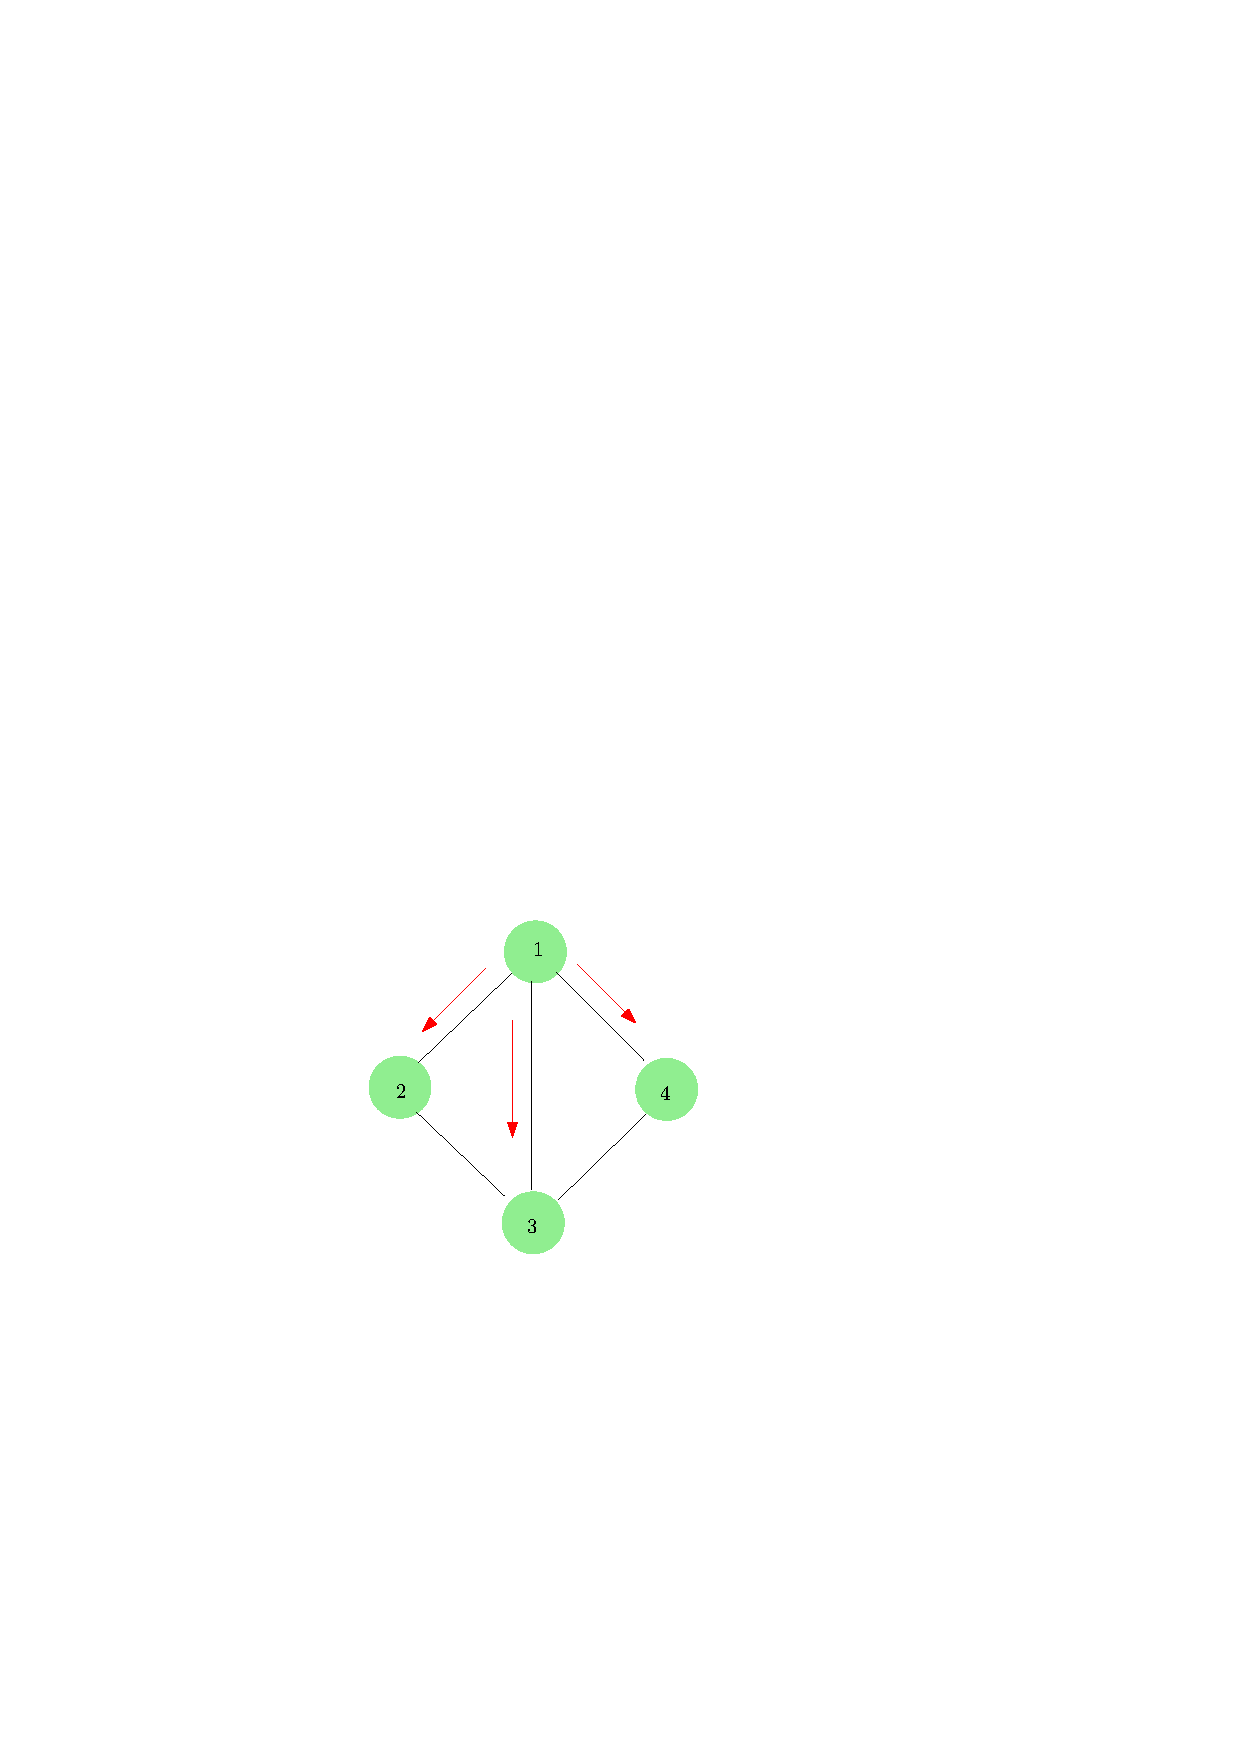
\includegraphics[width=0.32\textwidth]{chapters/background/images/echo/sync/notext_f0_1.pdf}}
    \subcaptionbox{Round Two}{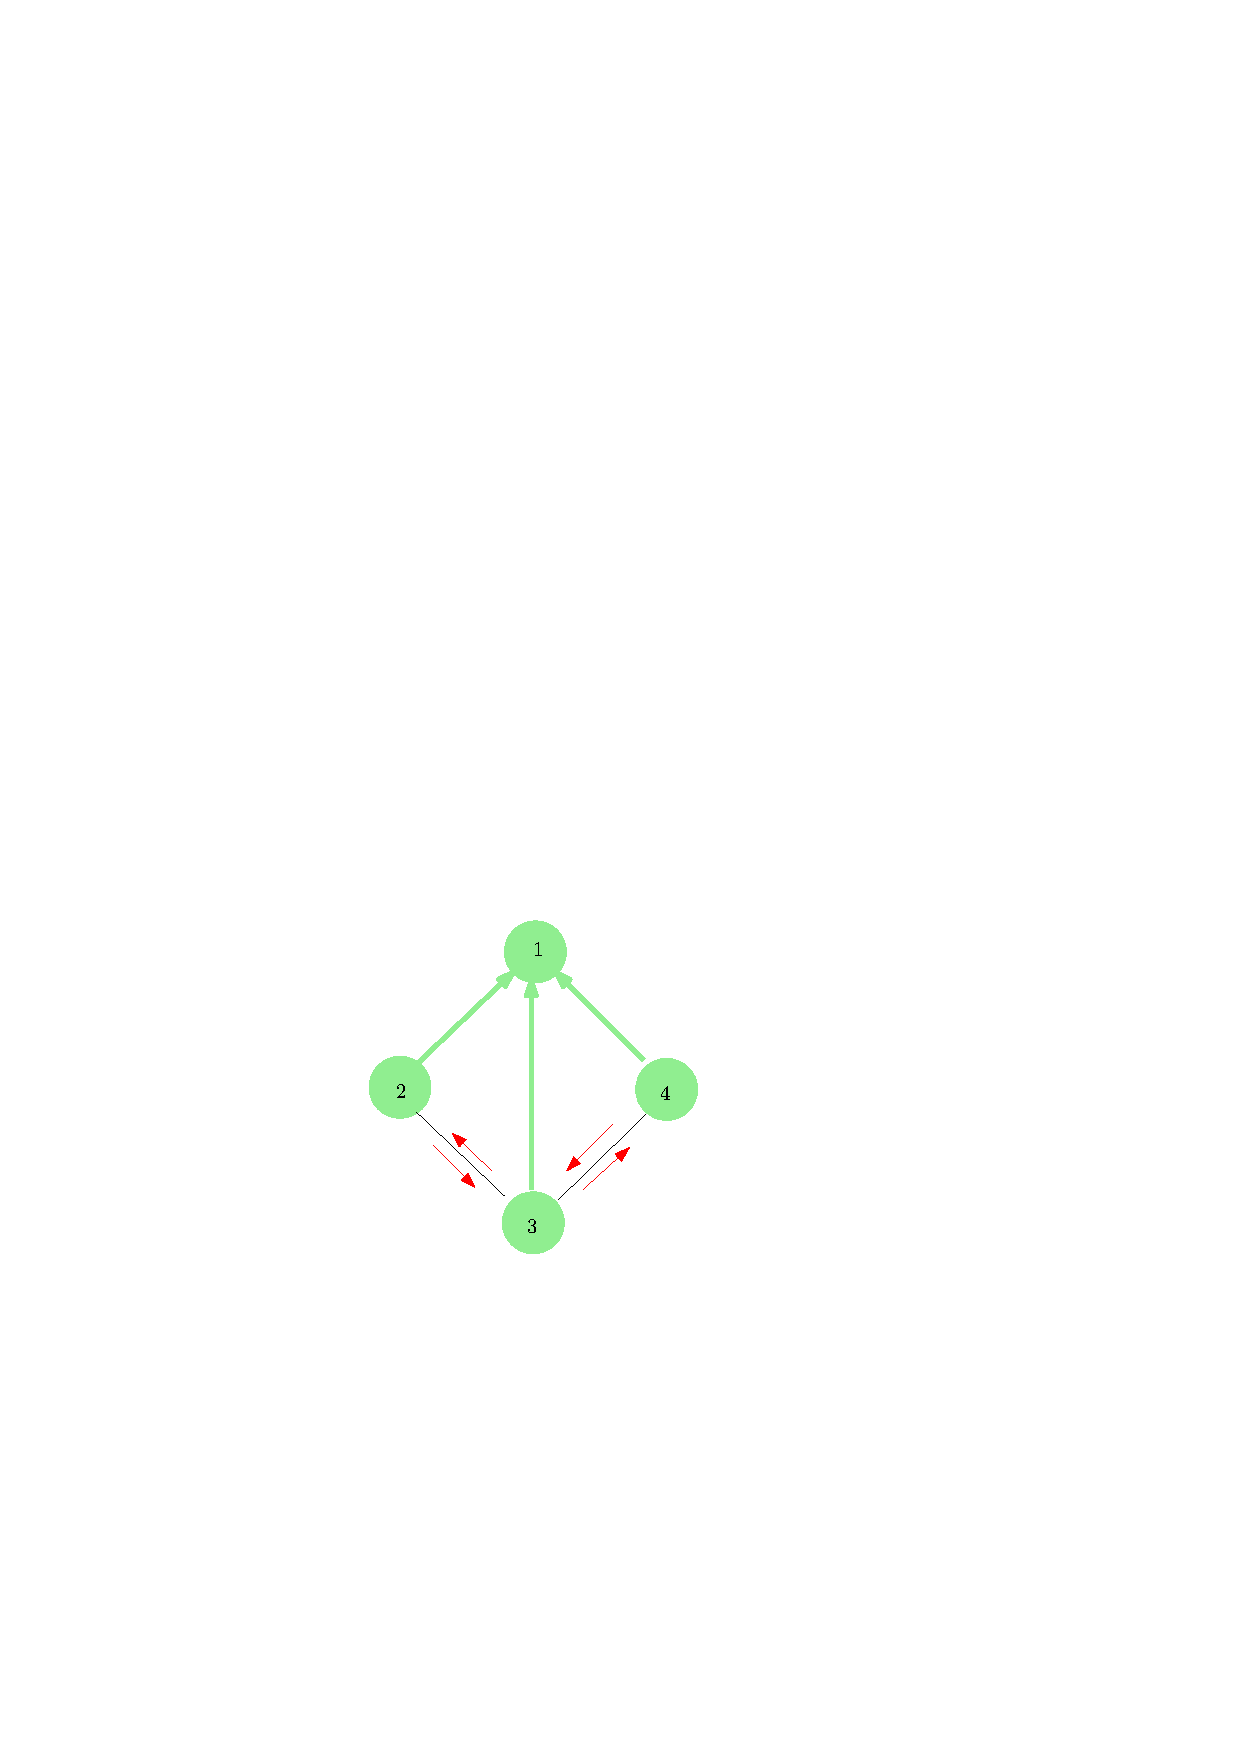
\includegraphics[width=0.32\textwidth]{chapters/background/images/echo/sync/notext_f0_2.pdf}}
    \subcaptionbox{Round Three}{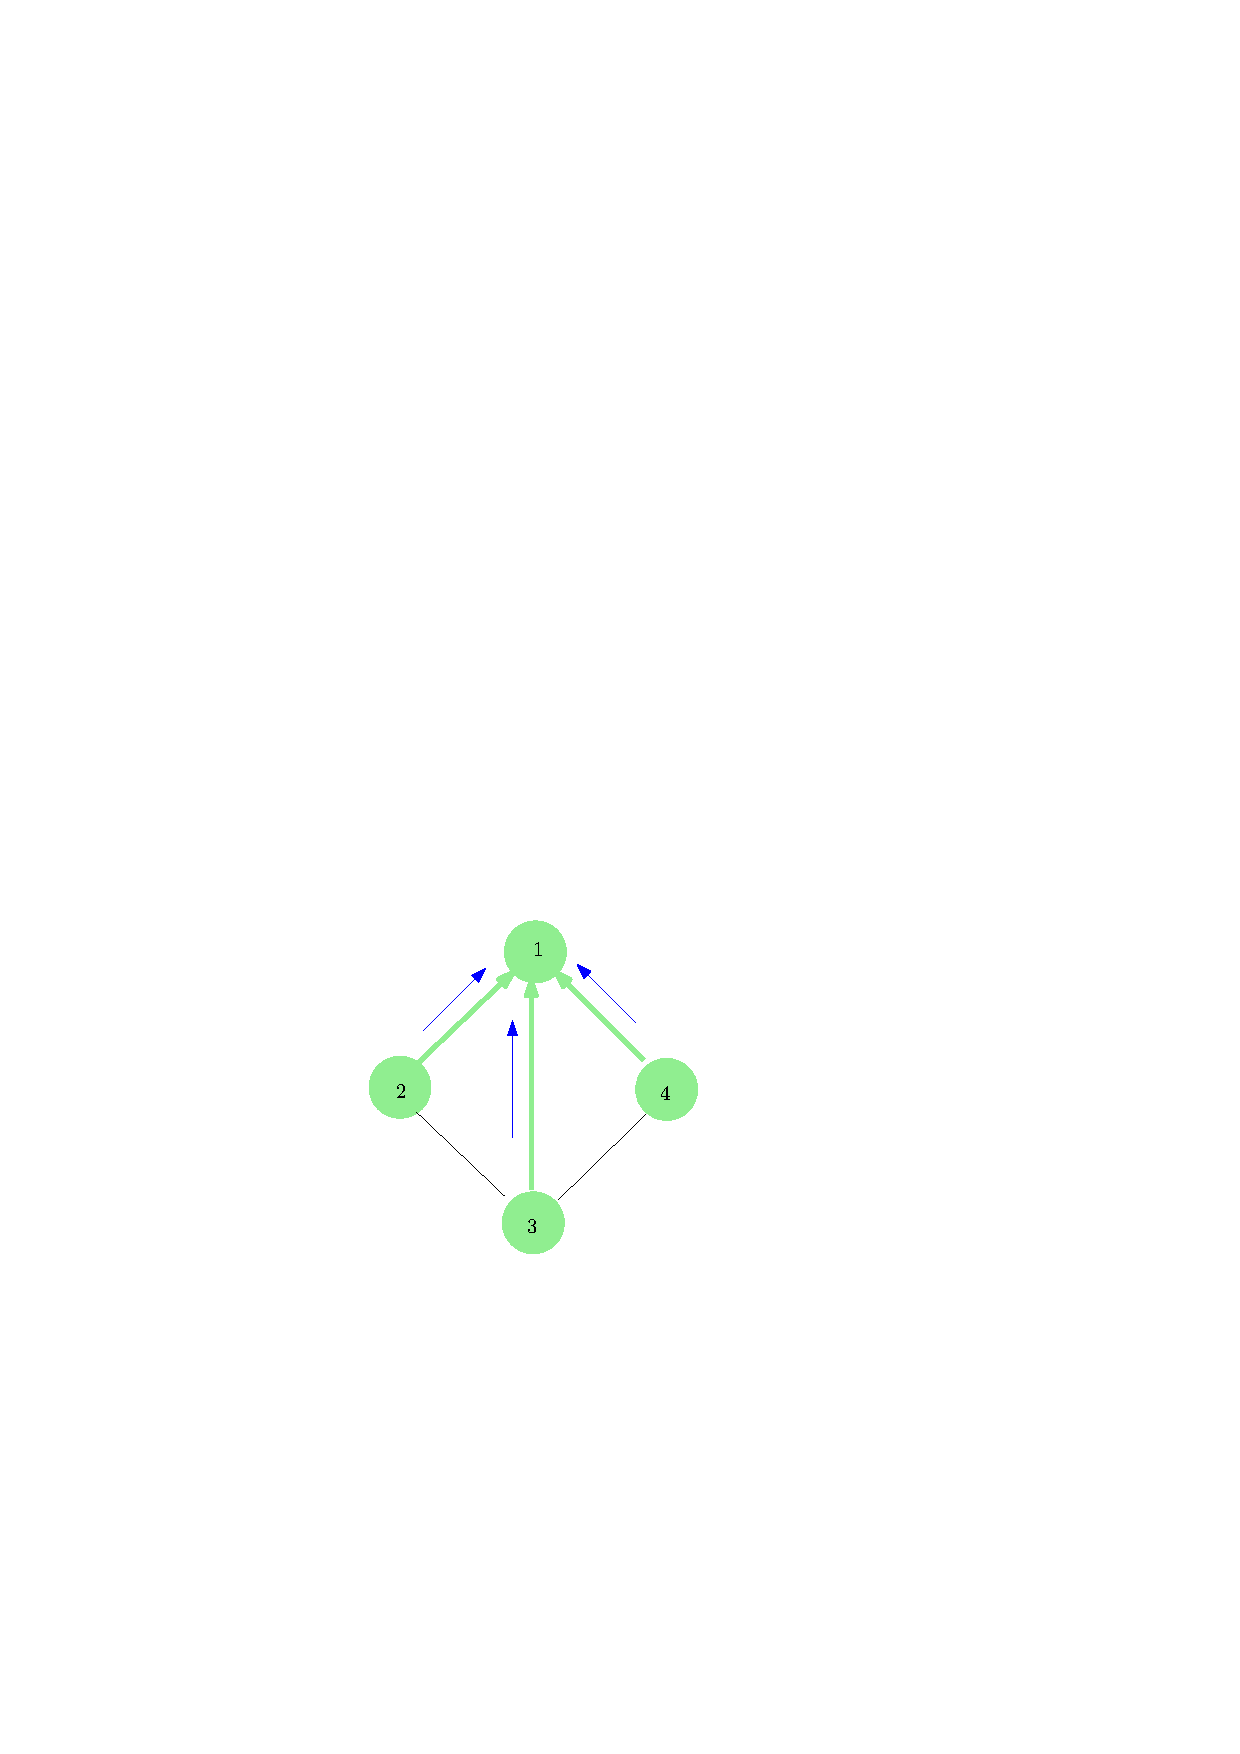
\includegraphics[width=0.32\textwidth]{chapters/background/images/echo/sync/notext_f0_3.pdf}}
    \caption[Progression of the synchronous \textsf{echo} algorithm]{Progression of the synchronous \textsf{echo} algorithm, starting from round zero before any messages are sent.  Arrows in red mean broadcast messages, while arrows in blue mean convergecast messages.}
    \label{fig:back:echosync}
\end{figure}

\begin{figure}[htbp]
    \centering
    \subcaptionbox{Round Zero}{\includegraphics[width=0.32\textwidth]{chapters/background/images/echo/async/notext_f0_0.pdf}}
    \subcaptionbox{Round One}{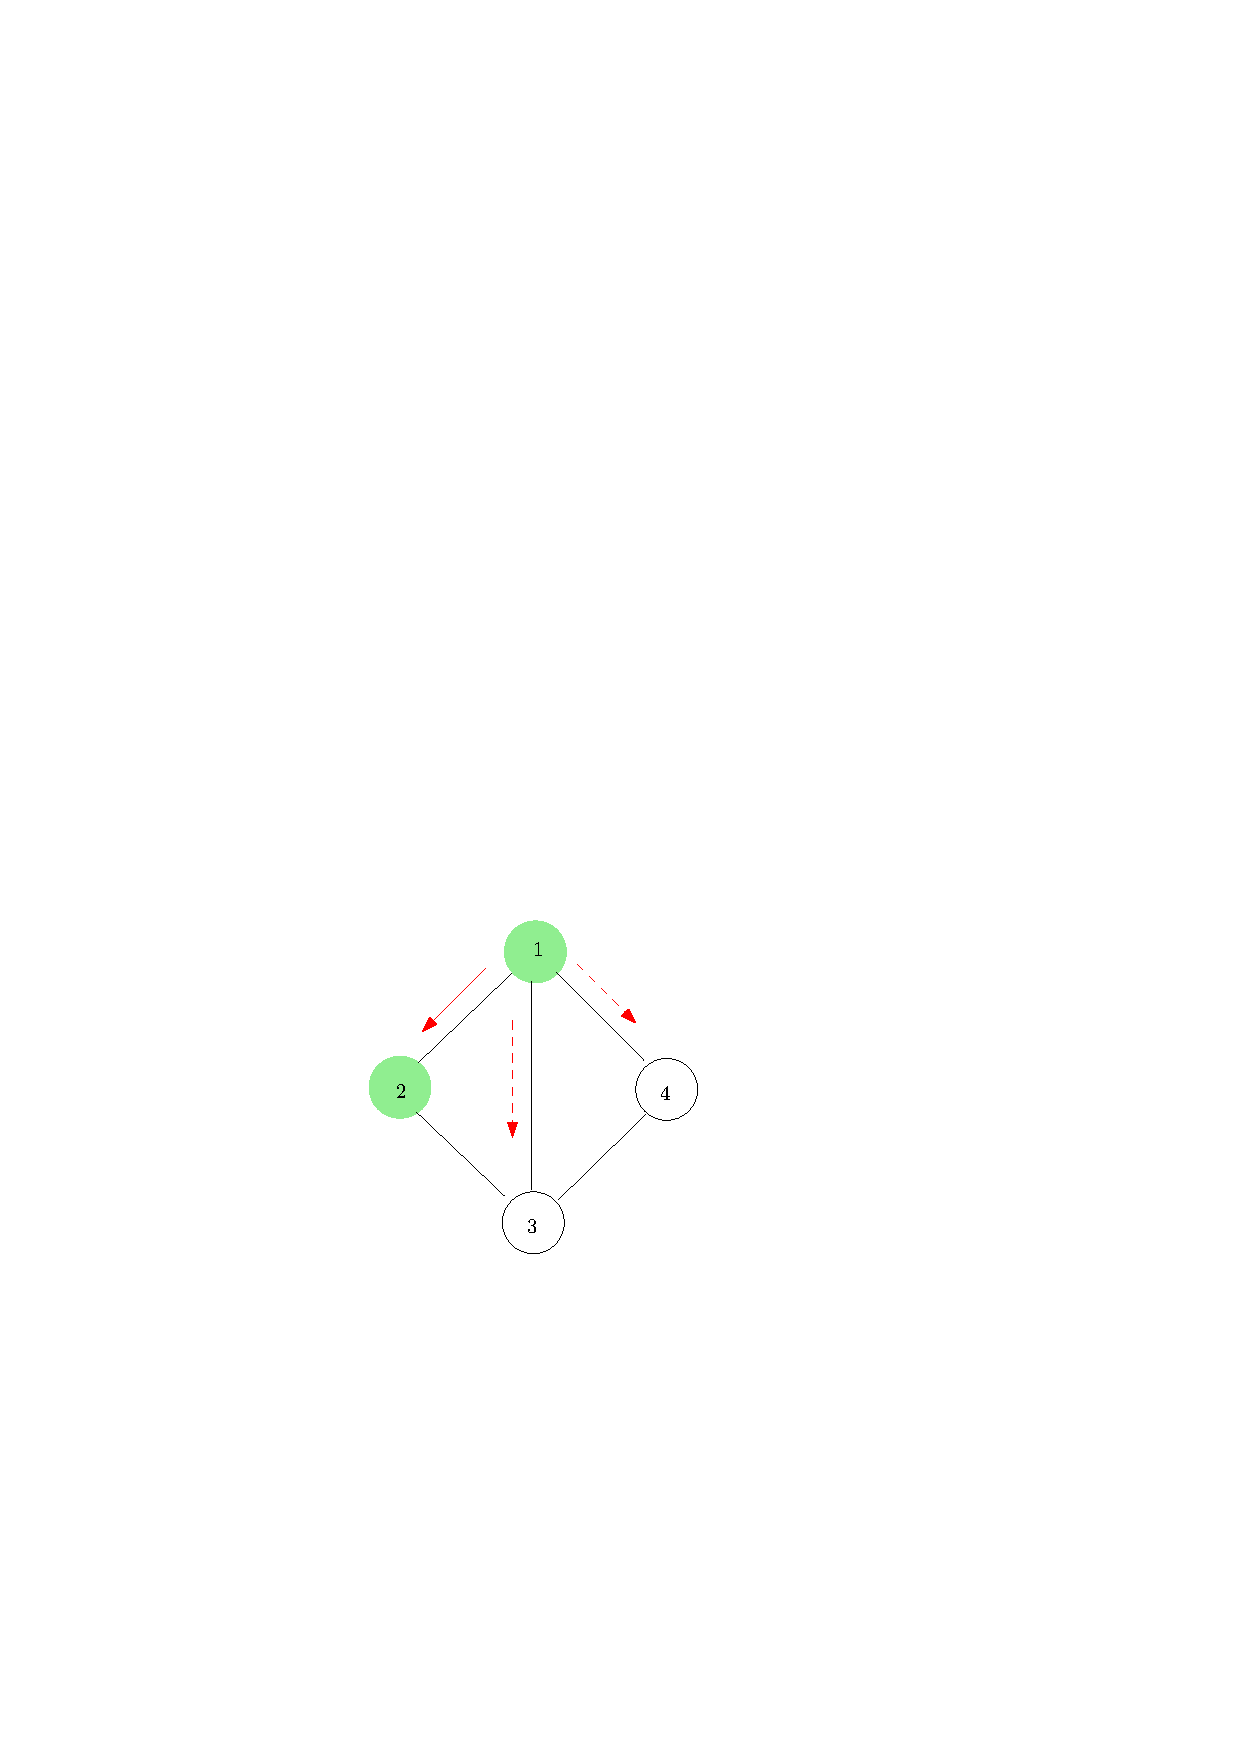
\includegraphics[width=0.32\textwidth]{chapters/background/images/echo/async/notext_f0_1.pdf}}
    \subcaptionbox{Round Two}{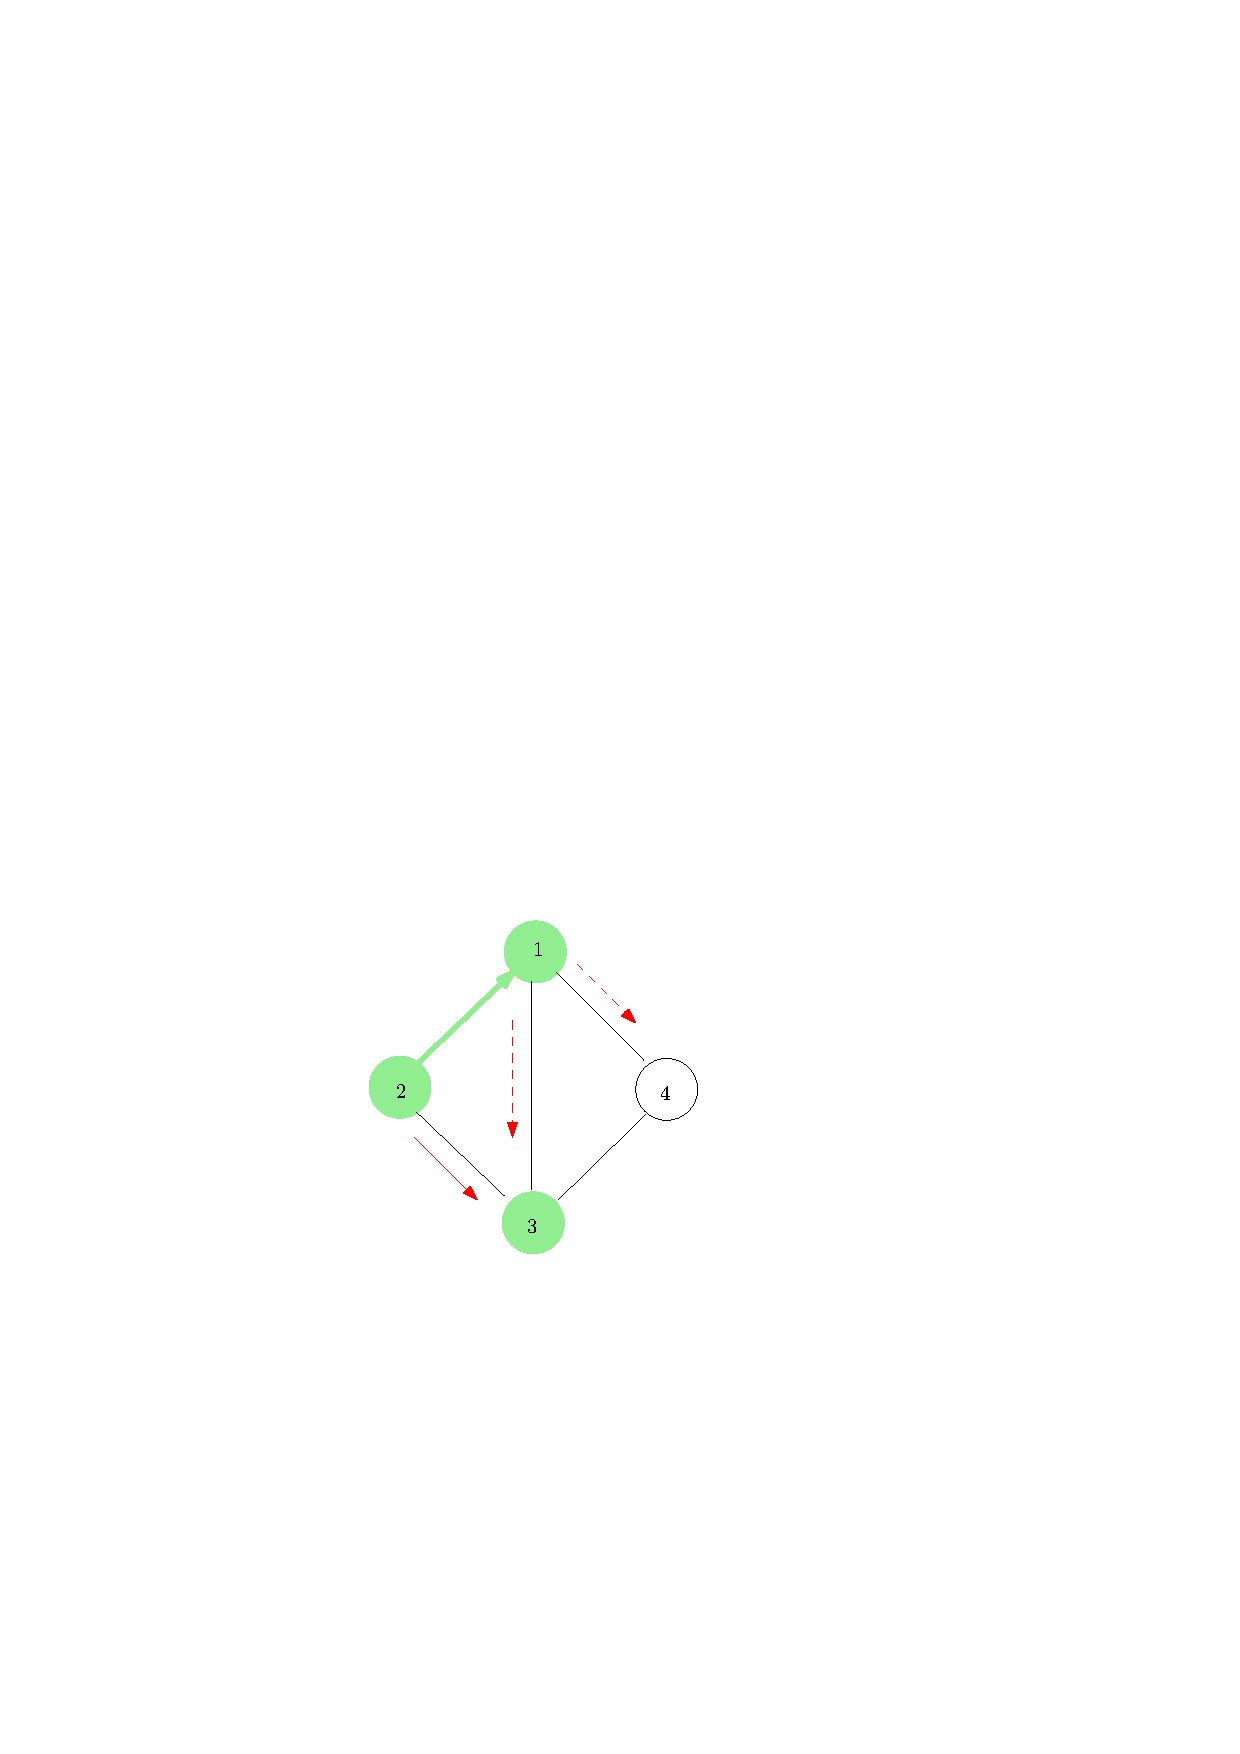
\includegraphics[width=0.32\textwidth]{chapters/background/images/echo/async/notext_f0_2.pdf}}
    \subcaptionbox{Round Three\label{fig:back:echoasync:3}}{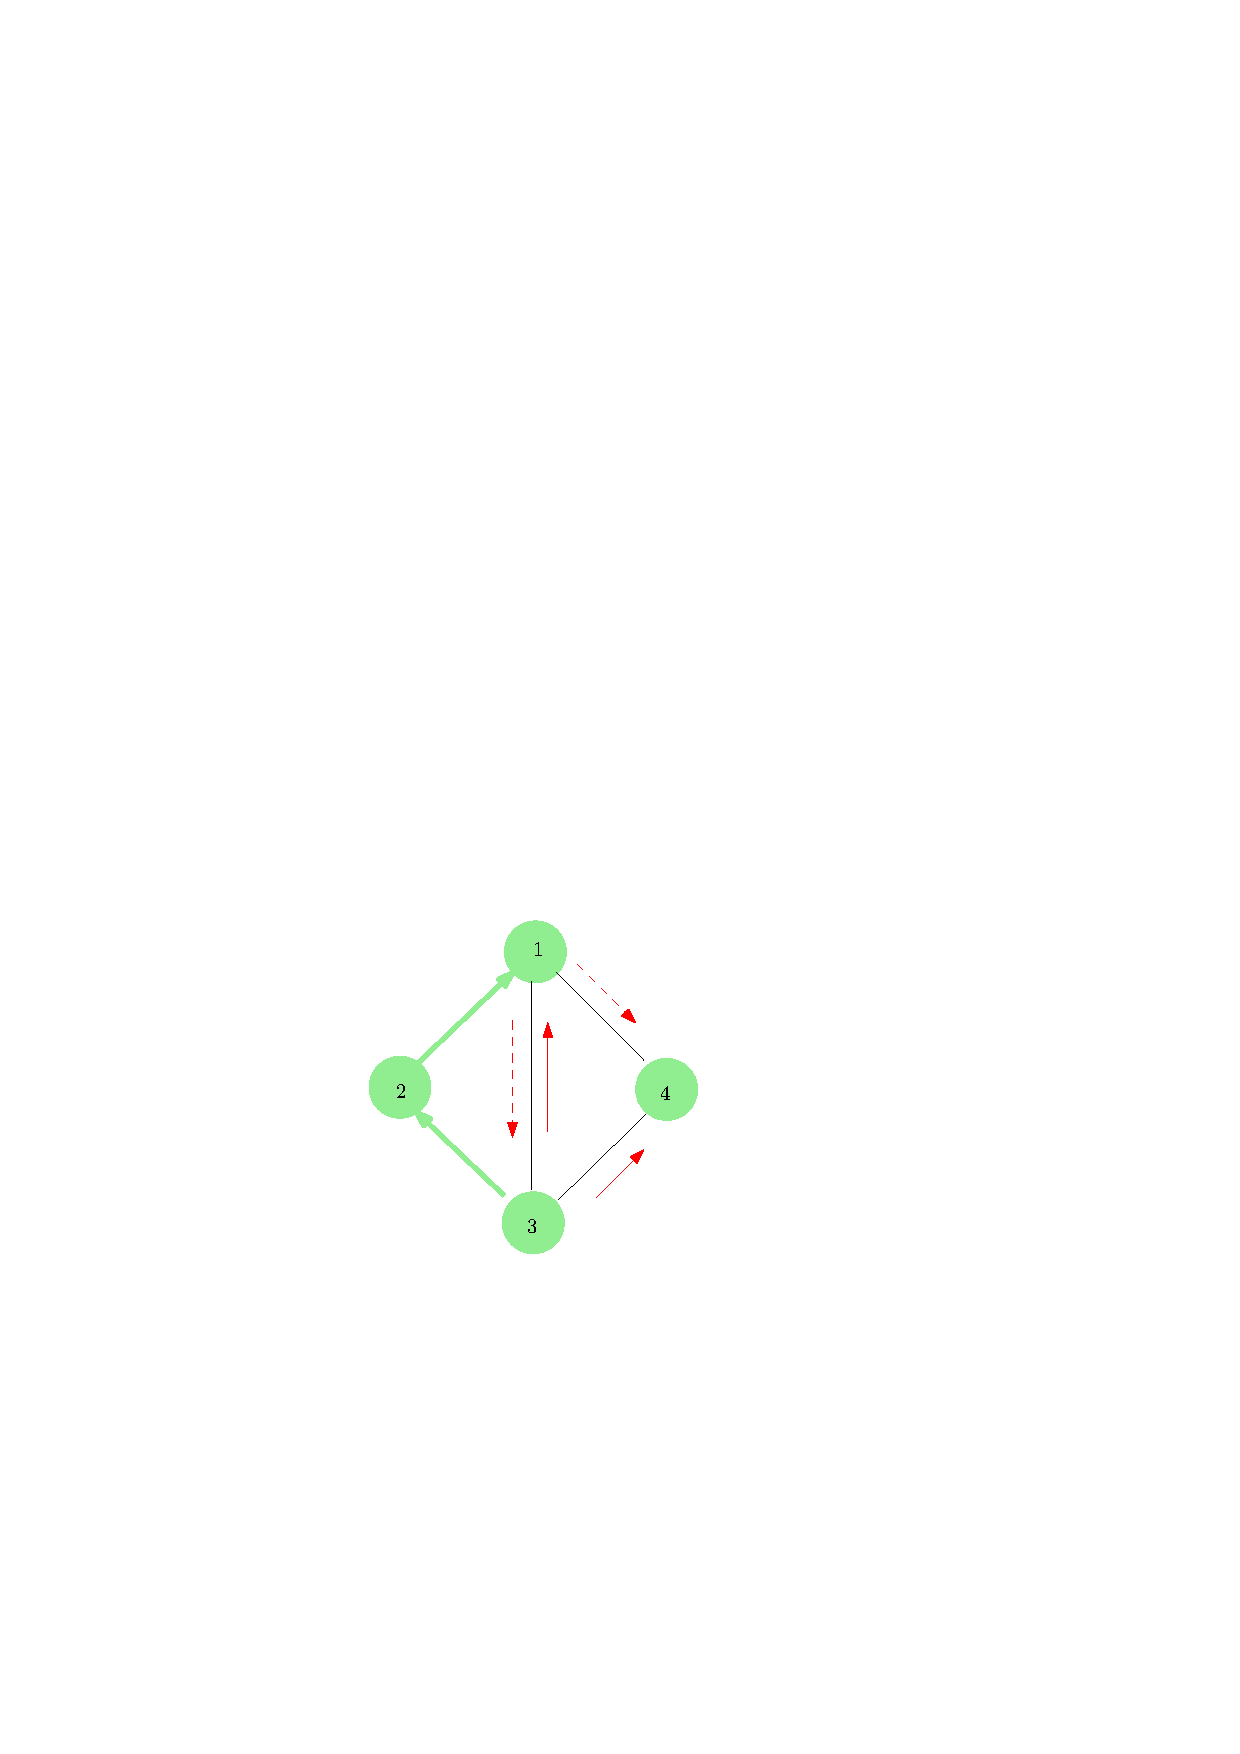
\includegraphics[width=0.32\textwidth]{chapters/background/images/echo/async/notext_f0_3.pdf}}
    \subcaptionbox{Round Four}{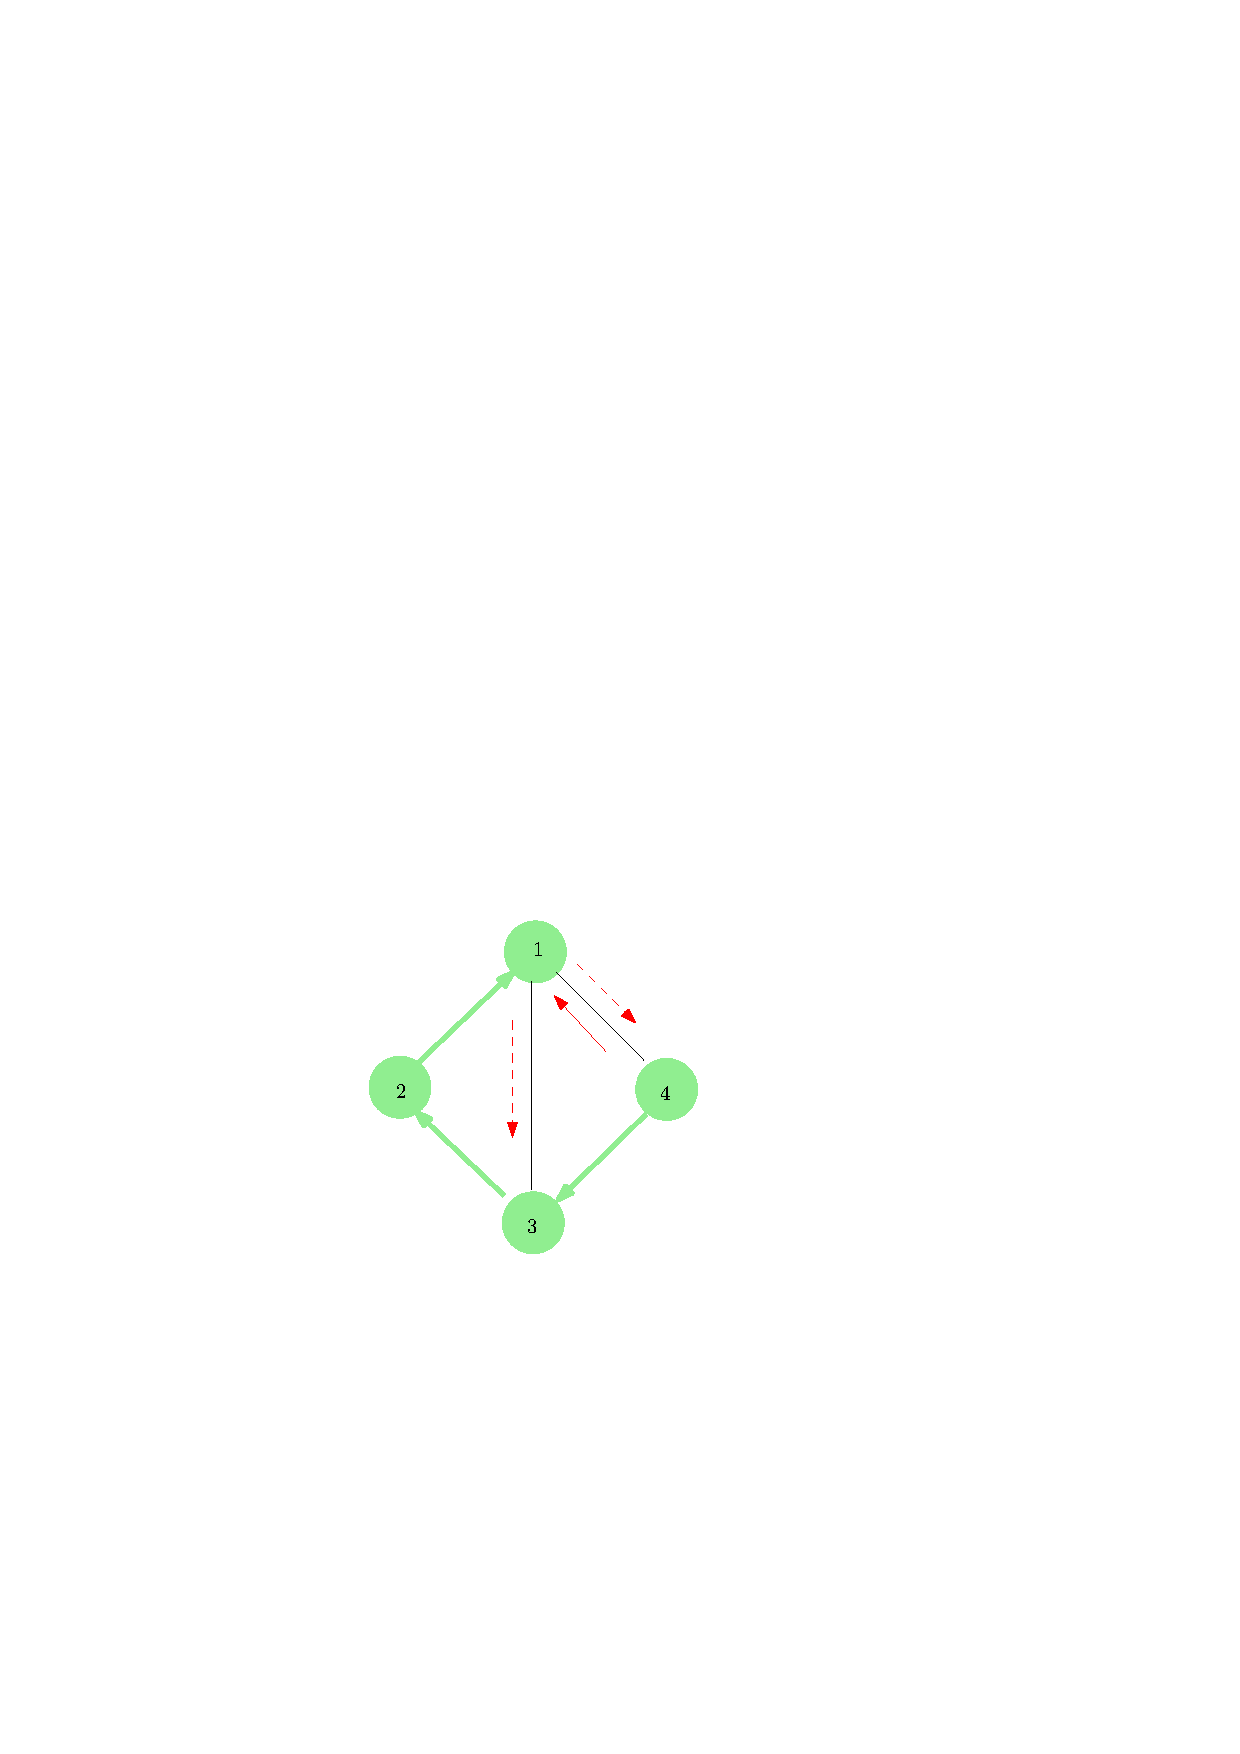
\includegraphics[width=0.32\textwidth]{chapters/background/images/echo/async/notext_f0_4.pdf}}
    \subcaptionbox{Round Five}{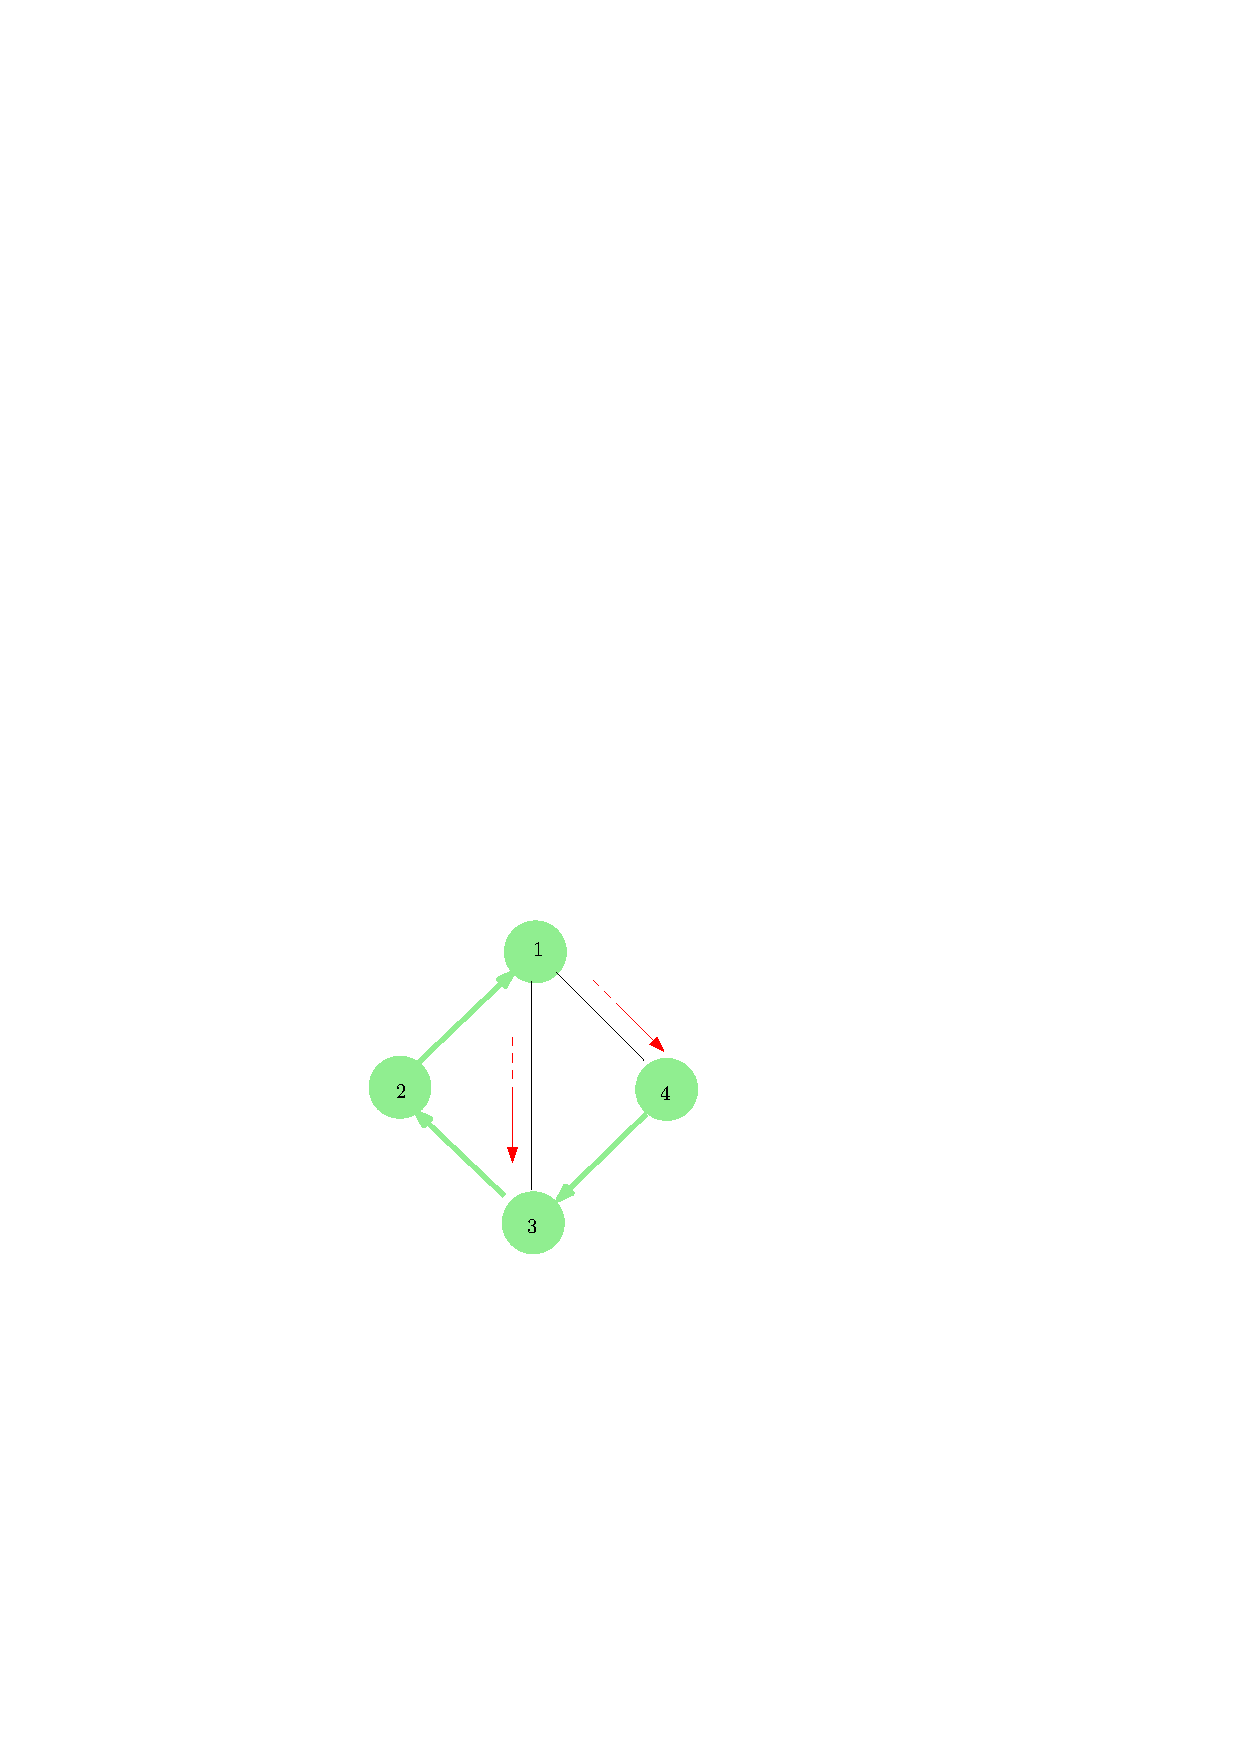
\includegraphics[width=0.32\textwidth]{chapters/background/images/echo/async/notext_f0_5.pdf}}
    \subcaptionbox{Round Six}{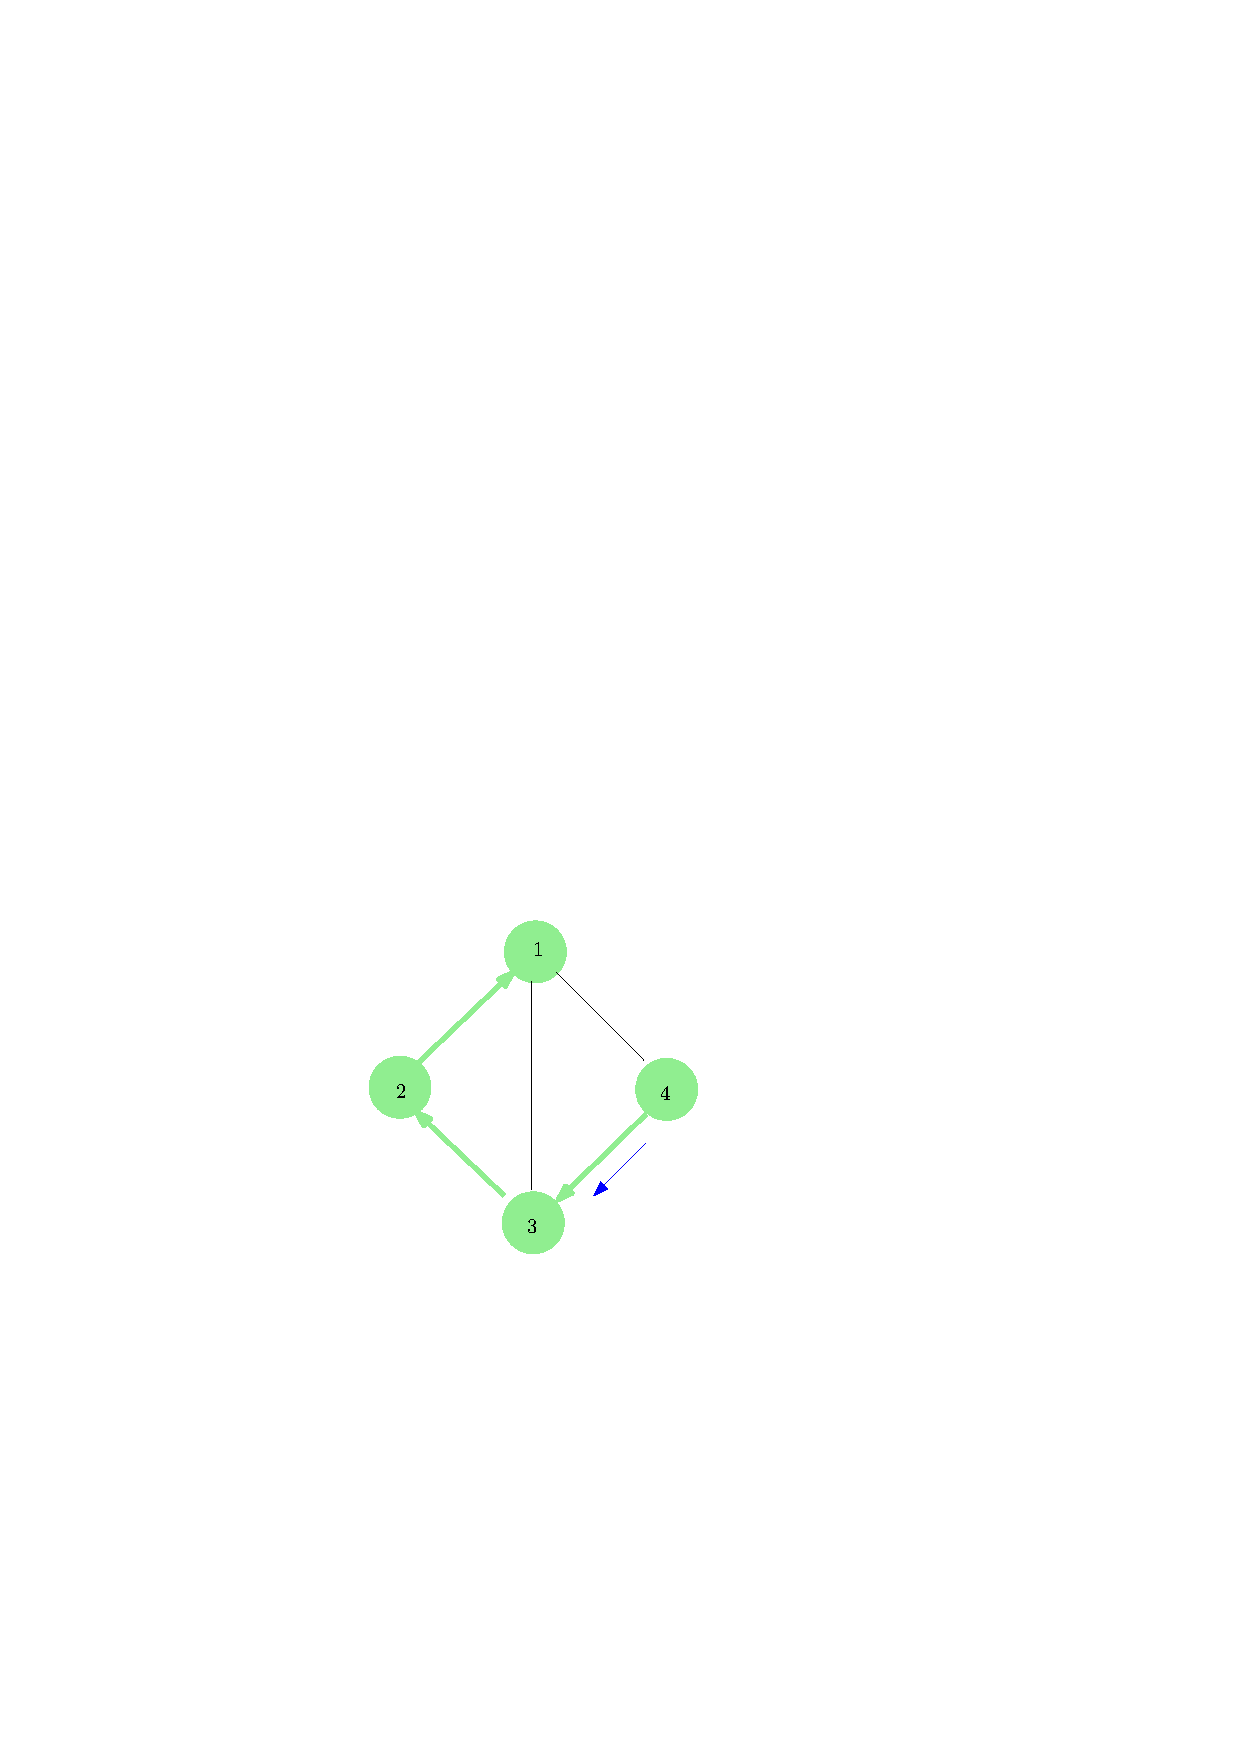
\includegraphics[width=0.32\textwidth]{chapters/background/images/echo/async/notext_f0_6.pdf}}
    \subcaptionbox{Round Seven}{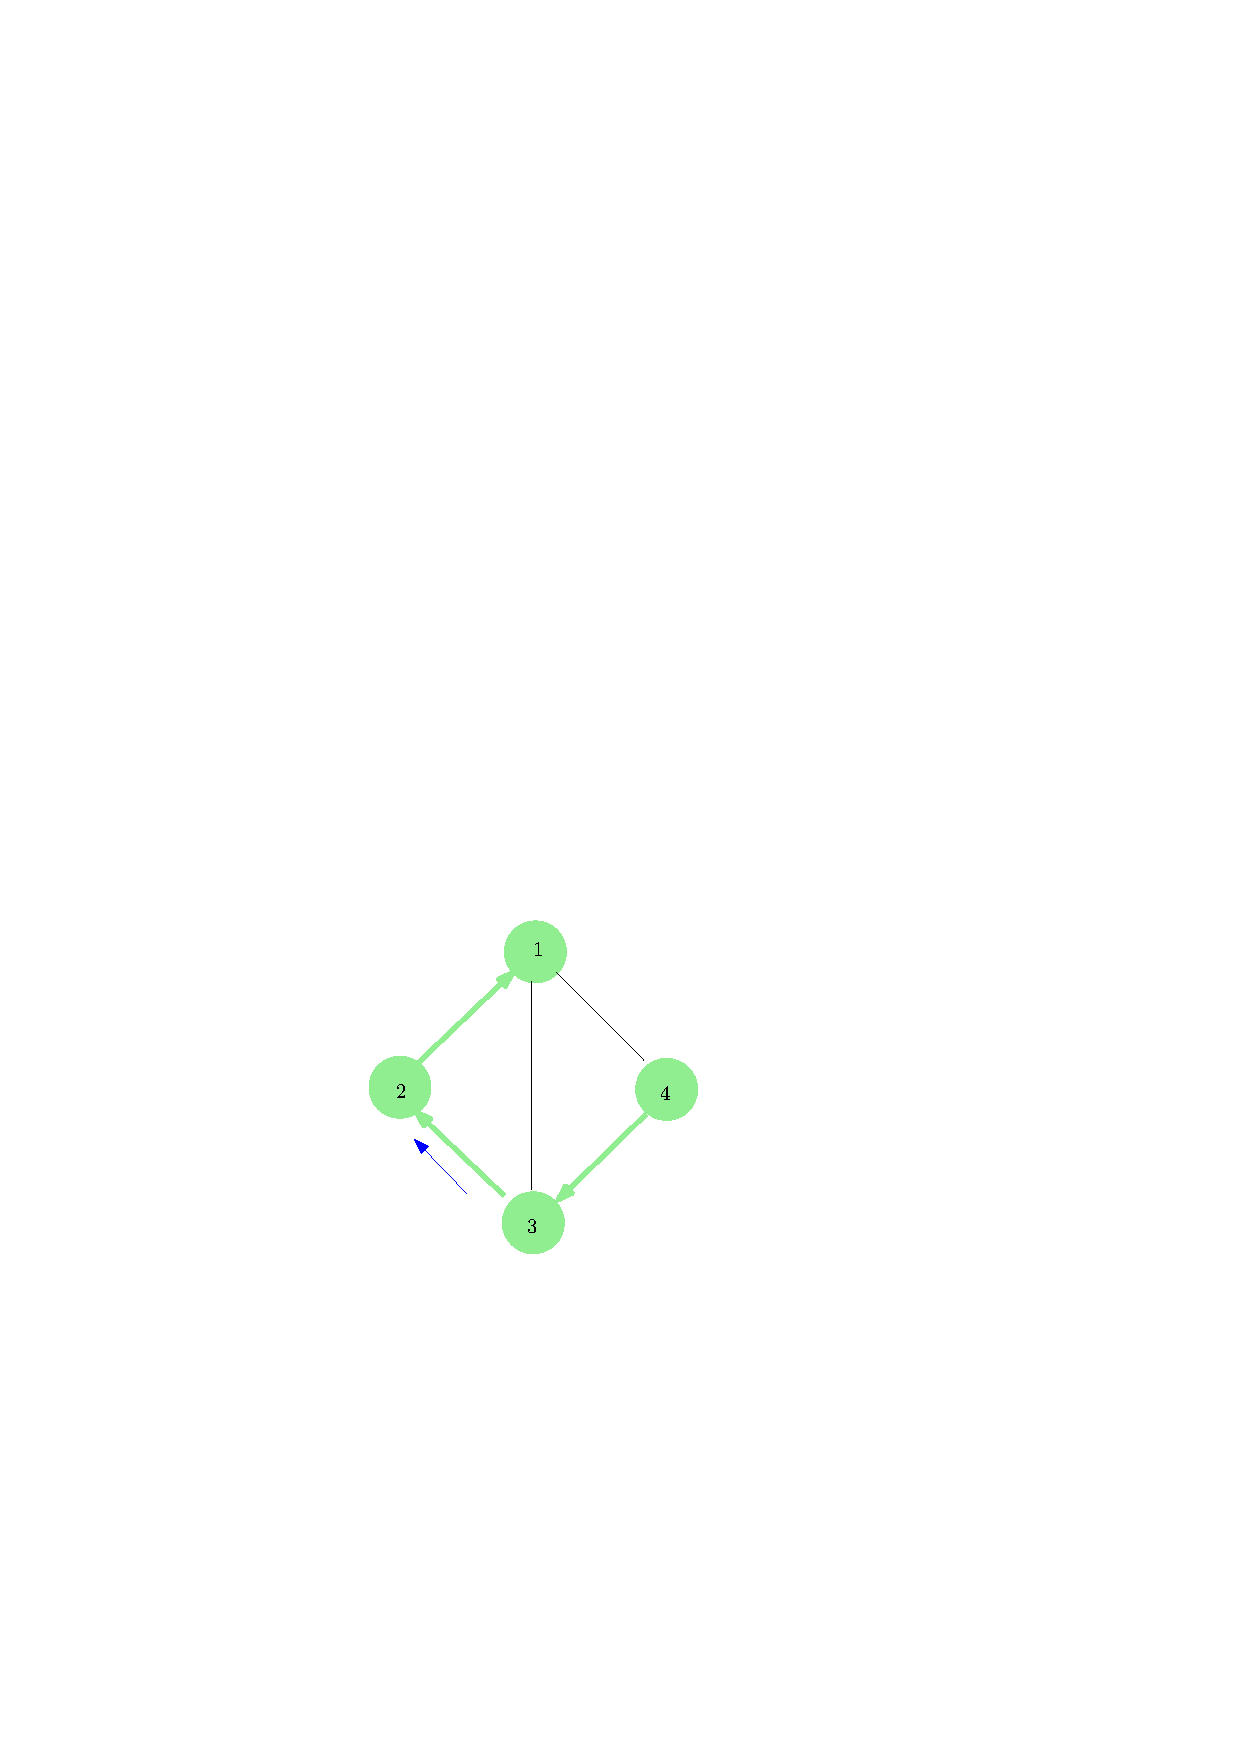
\includegraphics[width=0.32\textwidth]{chapters/background/images/echo/async/notext_f0_7.pdf}}
    \subcaptionbox{Round Eight}{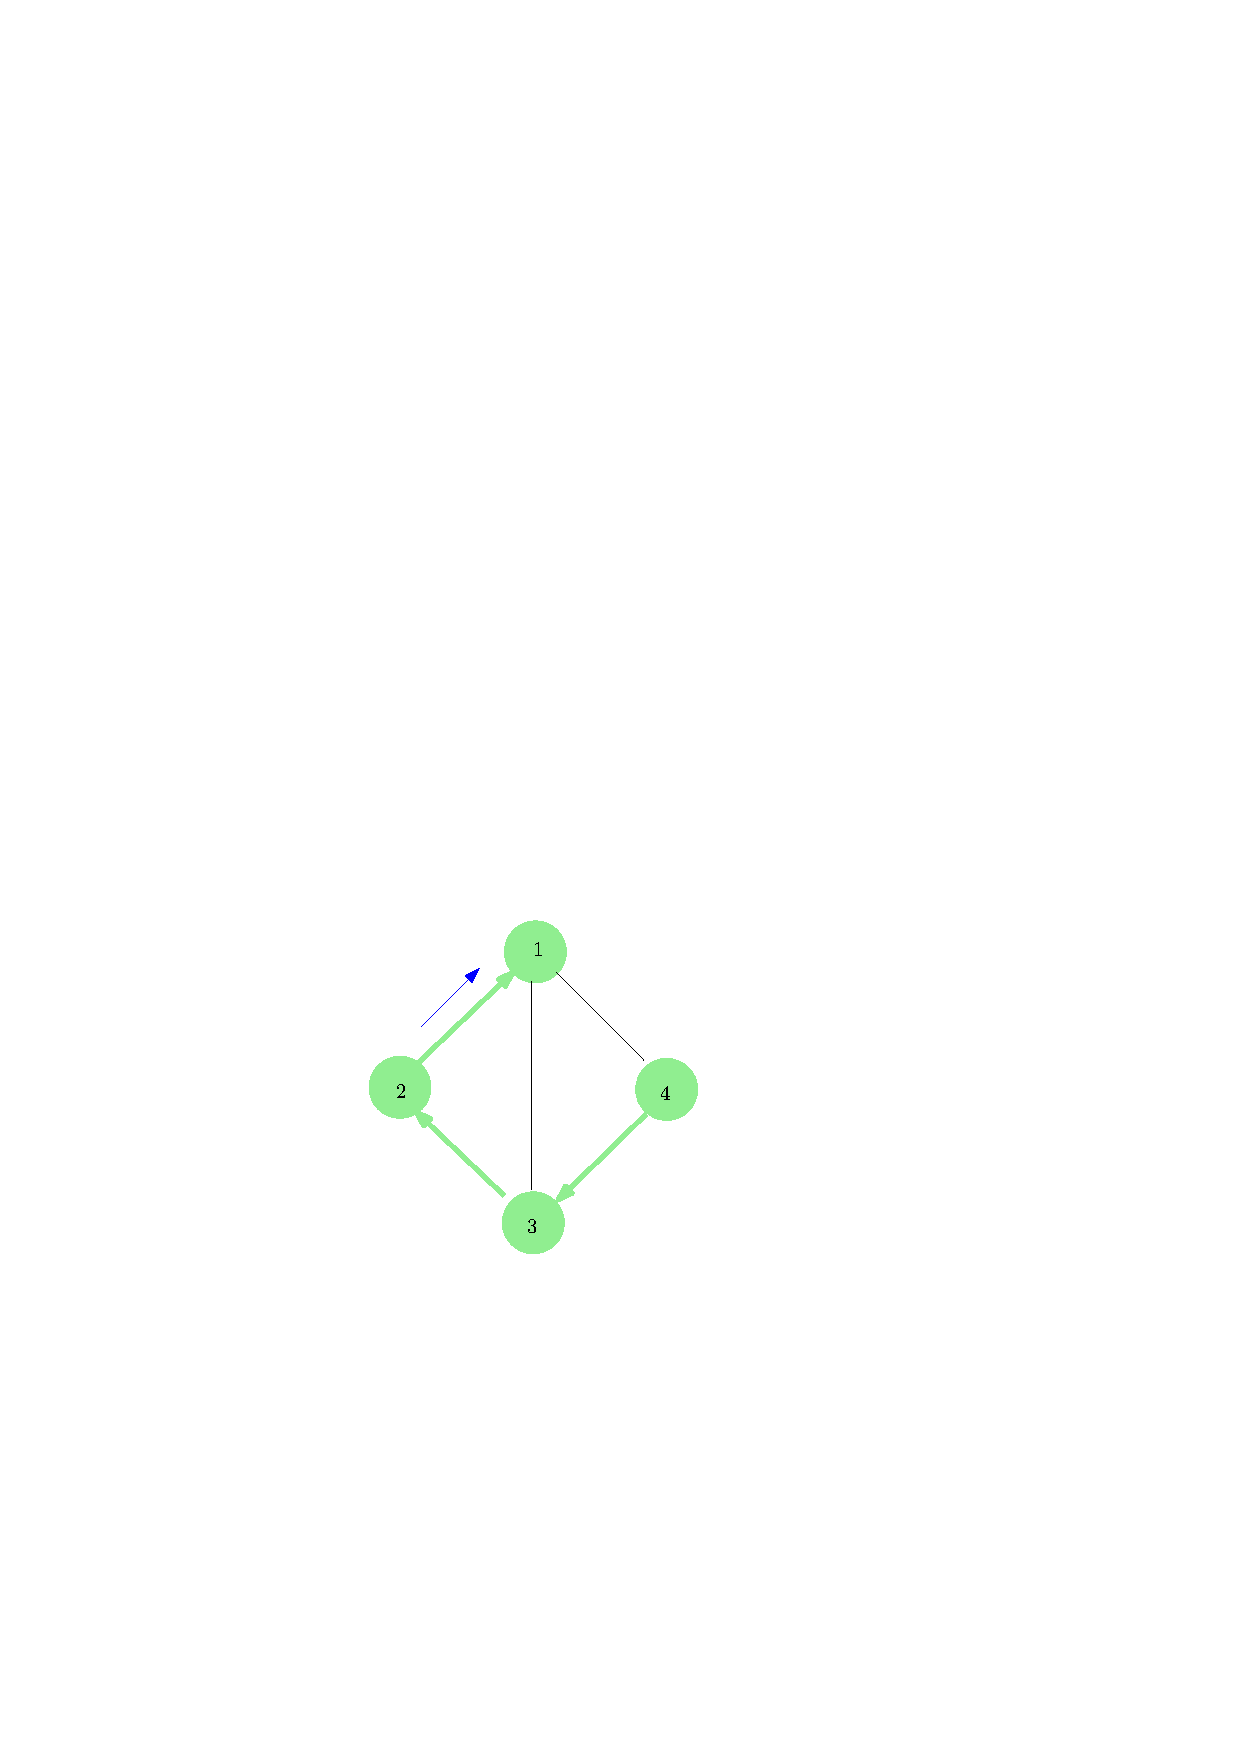
\includegraphics[width=0.32\textwidth]{chapters/background/images/echo/async/notext_f0_8.pdf}}
    \caption[Progression of the asynchronous \textsf{echo} algorithm]{Progression of the asynchronous \textsf{echo} algorithm, starting from round zero before any messages are sent.  Arrows in red mean broadcast messages, while arrows in blue mean convergecast messages.  Despite node 1 being the initiator node, node 4 considers node 3 to be its parent because it first receives a broadcast message from node 3.}
    \label{fig:back:echoasync}
\end{figure}

In the synchronous case, all messages sent out are received simultaneously, and all nodes proceed through their rounds together.  In the asynchronous case, however, messages may arrive at arbitrary times, and nodes proceed through their rounds entirely independently of one another.  The round numbers in the figure mark the point where at least one message has been received by a node.  The nodes react to messages as they arrive, and might do nothing for a time while other nodes are working if no new messages arrive during that time.  Under the asynchronous model, depending on communications topology and speeds, it is possible for the first broadcast message to reach a process to have followed a less direct route from the initiator than otherwise might be possible.  Exactly this is seen in \cref{fig:back:echoasync:3}, where node 4 first receives a message from node 3 (and thus marks node 3 as its parent), despite a direct connection to the initiator, node 1.
\section{\label{sec:back:cml}\glsfmtlong{cml-glossary}}

While parallelism is often the best (perhaps only) way to achieve improvements in execution time for different algorithms once an efficient sequential implementation has been created, it is a notoriously challenging affair \cite{Shun2017}.  When working at the level of directly manipulating threads, such as using the pthreads found in POSIX-compliant operating systems, programmers are exposed to a high level of risk of inadvertently introducing concurrency bugs, such as data races, deadlocks and livelocks.  A panoply of approaches to overcoming this challenge, both theoretical and practical, have been proposed and developed over the years, with varying degrees of success, \eg{} \cite{Boyapati2002,Bocq2012,Seinstra2004}.  Many, perhaps most, large-scale programming languages that use a runtime include some form of parallelism simplification within their standard libraries, \eg{} the Executor system in Java \cite[Ch. 4]{Fernandez2012}, and Swift \& Objective-C's Grand Central Dispatch \cite{Maskrey2018}.

Most simplifications fairly directly target either data-parallelism by simultaneously applying the same operation over multiple elements in arrays, \eg{} SIMD instructions in CPUs \cite{Hughes2015}; or task-parallelism by making provisions for the fork-join model \cite{McCool2012}.  These simplifications can be very useful, but not all instances of parallelism fit neatly into their models.  Algorithms that are well-modelled by the \Gls{csp} and \Gls{actor} models, such as those explicitly centred around concepts of message passing, are not necessarily easy to express using either SIMD or fork-join instructions.

\Gls{cml} \cite{Reppy1991,Panangaden1997} is an approach to concurrent programming originally developed by John Reppy (based on his earlier `Pegasus Meta-Language' \cite{Reppy1988}).  \Gls{cml} was created to provide a framework for creating concurrent programs with synchronous communications on single-core machines,\footnote{In fact, the original implementation \emph{relied} on the fact that the processor was single-core under-the-covers.} and was later extended to permit parallelism \cite{Reppy2009a}.  It was created originally as a library in Standard ML of New Jersey (where ML refers to the earlier programming language \textit{Meta Language}), whence the ML part of the name, but its concepts have subsequently appeared elsewhere.  The basic concept of communicating via channels has experienced a renaissance in recent years, likely due at least in part to its inclusion as a core feature of Go \cite{Meyerson2014}, but \gls{cml} has a more advanced system that Go (at the time of writing) does not fully support.

\Gls{cml} is designed to avoid many of the problems with concurrency that arise in traditional sequential programming, where the use of locks, mutexes and semaphores etc. are frequently required, and often lead to the potential introduction of problems such live-/deadlocks, data races and extreme resource contention.  This is achieved by changing the approach to concurrent programming to one of logically separate, internally sequential processing elements that share data as required by `passing messages'\footnote{This is the logical concept, but there is not strictly any specific required software implementation.} between themselves.  In \gls{cml}, these logical processing elements are referred to as threads, and they exchange messages over channels \emph{synchronously} (called \emph{rendezvous}), \ie{} there is a temporal overlap between one thread offering to send, and another to receive, over the same channel, and the first to offer blocks until the second makes its offer.  When two processes are offering appropriately on either side of an exchange, rendezvous takes place.

Reppy describes a concurrent program as one that supports multiple sequential sub-programs conceptually executing in parallel separately, but interacting through shared resources to achieve a common goal.  \Gls{cml} is concerned with the scenario where said interactions are explicit, and in order to facilitate that \enquote{\gls{cml} takes the unique approach of supporting \emph{higher-order concurrent programming}} (emphasis Reppy's), whereby communication and synchronisation are made into first-class members of the language, similar to how functional programming languages made functions into first-class members of themselves \cite[Preface]{Reppy2007}.

\begin{anfxerror}{Expand this?}
Describe more of how \gls{cml} works?  Is there not something in the gcol chapter that can be shifted into here, at least?
\end{anfxerror}
\section{\label{sec:back:mc}\Glsfmtname{mc}/\glsfmtname{ps}}

\emph{\Gls{mc}}, also known as \emph{\gls{ps}} (the two terms are generally used interchangeably), is a bio-inspired model of computing created by Gheorghe Păun in the late 1990s \cite{tPaun98a,Paun2000}.  It was originally conceived of by considering the process of chemical reactions and exchanges that occur inside living biological cells and the membranes within, and regarding this process as a form of computation.  \Gls{mc} was identified in 2016 by the National Research Council of Canada as \textcquote[][p. 17]{Wiseman2016}{a rigorous and comprehensive framework that provides a parallel distributed framework with flexible evolution rules.}

\citeauthor{Paun2002} describes \gls{mc} as:
\blockcquote[][p.~VII]{Paun2002}{Membrane computing is a branch of natural computing which abstracts from the structure and the functioning of living cells. In the basic model, the membrane systems -- also called P systems -- are distributed parallel computing devices, processing multisets of objects, synchronously, in the compartments delimited by a membrane structure. The objects, which correspond to chemicals evolving in the compartments of a cell, can also pass through membranes. The membranes form a hierarchical structure --- they can be dissolved, divided, created, and their permeability can be modified. A sequence of transitions between configurations of a system forms a computation. The result of a halting computation is the number of objects present at the end of the computation in a specified membrane, called the output membrane. The objects can also have a structure of their own that can be described by strings over a given alphabet of basic molecules - then the result of a computation is a set of strings.}

\begin{anfxerror}{P systems Diagram?}
Include a copy of the membrane layout diagram from Paun?
\end{anfxerror}

\Gls{ps} works analogously to a typical modern electronic computer, in that the system stores data and processes \& updates those data based on a predefined program, with a view to arriving at a computable answer based on the starting state and any inputs to the system \cite{Paun2002,Paun2010b}.  In classical \gls{ps}, the data are multisets of symbols, representing various chemicals and their quantities.  These are found inside one or more \emph{cells},\footnote{Loosely based on real biological cells.} which (to a certain extent at least) form a hybrid between main memory and the processing units of a computer.  The instructions of the program itself are provided by \emph{rules}, which specify transformations of objects and interactions with the surrounding environment and other membranes or cells.

There are now, broadly, three main families of \gls{ps} variants:  \gls{clps} \cite{Paun2001,Paun2002}, \gls{tlps} \cite{tMaPaPaRo01a,Martin-Vide2003} and \gls{snps} \cite{Ionescu2006}.\footnote{Several other variants have been created, but most are used infrequently, if ever.  Most recent work in \gls{mc} has focused on sub-variants of \gls{clps}, \gls{tlps}, \gls{snps} and \gls{cps}.}  \Gls{clps} is the direct descendant of the original classical \gls{ps}, and sees objects compartmented into \emph{membranes}, which are arranged in a graphical tree structure with the outermost \emph{skin} membrane -- which separates the cell from its environment -- as the root of the tree.  In most variants, objects can evolve inside a membrane, but also be communicated between membranes (and the environment).  Furthermore, membranes can \emph{divide} or \emph{dissolve} themselves, and may have one or more special properties, such as \emph{polarization} \cite{Paun1999a}.

On the other hand, \gls{tlps} and \gls{snps} both arrange their computing compartments -- named \emph{cells} or \emph{neurons}, respectively -- as nodes in arbitrary digraphs, with the edges between them representing connecting channels or synapses.  Whereas \gls{clps} emphasises the evolution of multisets of objects inside membranes of a given cell, \gls{tlps} and \gls{snps} emphasise communication between separate cells/neurons, and might not include any capacity for internal evolution inside cells.  If new objects are required, they are imported via communication with the environment, which possesses an unlimited number of all objects but has no rules of its own.

While \gls{tlps} have arbitrary alphabets, only one object is used in \gls{snps}, the \emph{spike}.  This means that \gls{tlps} are frequently much like \gls{clps} in that they have custom objects for each purpose, with the key difference (usually) being in the arrangement of the compartments/membranes/cells relative to each other and the choice between the two motivated primarily by which one better fits the computation to be modelled.

Conversely, \gls{snps} represent everything through the use of differing quantities of the spike, kept in different neurons.  This means that it can be more complex to model certain problems, but also arguably means that \gls{snps} are, \textit{prima facie}, closer to Lambda Calculus \cite{Barendregt1984} and Church Numerals (see \eg{} \cite{Koopman2014,Hinze2005}), as well as Register Machines (see \eg{} \cite{Korec1996}) (and indeed Register Machines have been simulated with \gls{snps} \cite{Pan2010}).  All three main types of \gls{ps}, in some form, have been proven Turing-universal though \cite{Bernardini2005,Chen2008,Freund2005}, so all three should be capable of expressing the same computations in different forms.  Furthermore, because \gls{snps} can be easily represented numerically, they lend themselves well to vector/matrix representations \cite{Zeng2010,Martinez-del-Amor2021,Gheorghe2021,Hu2016}.  This means that, potentially, \gls{snps} implementations can take advantage of high-performance techniques such as directly using \gls{blas} \& \gls{lapack} and/or \glspl{gpu} \cite{Aboy2019}.

Arguably, the most noteworthy and important aspects of \gls{ps} models are that:
\begin{inparaenum}[(i)]
\item They have no space limit.  That is, they contain an unbounded number of cells, objects and membranes;
\item Usually, across all cells and membranes, all rules that can be applied are applied, as many times as possible given the current number of objects available.
\end{inparaenum}
These two features mean that \gls{ps} have unbounded space and processing capacity, which can be used to solve traditionally computationally difficult problems relatively quickly \cite{Sosik2003,Jimenez2003,Paun1999a,Henderson2020}.  Most of these solutions, however, rely on trading time complexity for space complexity.  While this works in the theoretical framework, electronic simulations of the systems do not have access to unlimited instantaneous memory space, meaning many of the fast solutions are impractical with current real-world computers, \eg{} \cite{Cooper2019,Cooper2019a} \fxnote[inline]{[refs]} (see further \vref{sec:psystemsuses}).

\citeauthor{Valencia-Cabrera2019} said of this:
\blockcquote[][p.~213]{Valencia-Cabrera2019}{We do not know if we will have those machines able to solve NP-complete problems in polynomial time, in many cases even linear time, but \textins{that does} not necessarily mean we will have to wait until that moment in biochemical technology to find some relevant use of P systems. As Babbage kept working on his ideas, not simply waiting until the precise moment when Turing, Von Neumann, and their contemporaries witnessed the first electronic computers based on similar principles, membrane computing must keep moving, finding new ways to provide a step further.}

Nevertheless, modelling a problem in \gls{mc} can lead to new insights or improved formulations of solutions, as occurs in \cref{chap:nmp}.  For example, in \cite{GimelFarb2013a} (building on \cite{Gimelfarb2011}) \citeauthor{GimelFarb2013a} describe how formulating Symmetric Dynamic Programming \gls{sm} in terms of \gls{ps} led to finding a bug in the implementation, \textcquote[][p.~24]{GimelFarb2013a}{but also (and what is much more important) refactor this algorithm, based on our cell structure.  The result is a more robust and flexible version, which allows us to fine tune its parameters and enhance its capabilities, without rewriting it from scratch.}  Furthermore, as reported in \cite{Nicolescu2014b}, this exercise led directly to the creation of a new \gls{sm} algorithm, Concurrent Propagation \cite{Gimelfarb2012}.  \citeauthor{Pang2018} \cite{Pang2018} also claim significant benefits from modelling certain problems in a novel variant of \gls{enps} \cite{Pavel2010}, but it is unclear how much of the stated benefit compared to their baseline implementation arises instead from the use of a \gls{gpu}.

\subsection{Objects, Rules and Steps}
All known \gls{ps} types fundamentally operate on a similar basis:  One or more sets of rules -- \emph{\gls{ruleset}} -- are defined, describing how the \emph{objects} present in the system's compartments change at each \emph{step}.  As mentioned above, the objects are usually multisets of arbitrary symbolic \emph{atoms}, with the exceptions of \gls{snps} which uses the spike as its only symbol, and Numerical \gls{ps}, which uses ordinary numbers in place of atoms.  Certain systems may introduce other object types as required.

\Gls{ps} types normally operate synchronously and assume the presence of a global clock.  At each clock ``tick'', every compartment compares its extant objects and its \emph{evolution rules}, determines which rules are applicable given the current objects, and then deletes the objects used in the rules, replacing them with new ones as the rules dictate.  This process comprises a step.  The progressive execution of the system's rules over multiple steps is referred to as the system's evolution.

All \gls{ps} evolve, and therefore all types have evolution rules (though they may not be referred to as such).  Other types of rules are possible, including: \emph{dissolution} and \emph{division} rules in \gls{clps} and \gls{tlps}, where membranes either dissolve and release their objects into the their parent membrane, or replicate themselves (essentially performing mitosis) and distribute their contents among the new membranes; \emph{forgetting} rules in \gls{snps} whereby one or more copies of the spike are removed from a given neuron; or, splicing rules in Splicing \Gls{ps}\footnote{Particularly notable for working over strings of an alphabet, instead of multisets.} \cite[Ch.~8]{Paun2010b}.

All rules use the same basic model.  At the start of a step, they check if the necessary pre-conditions for the rule are met.  If they are, then any changes to the state of the system specified by the rule occur.  It is common for rules to remove or delete some objects in the relevant compartment, and instantiate new ones.  It is typically assumed that all objects are deleted or created instantaneously at the last moment of the rules' execution.

Generally, rules are specified in the form \textsc{\gls{lhs}} \(\rightarrow\) \textsc{\gls{rhs}}, where objects to be removed (the presence of which are therefore a precondition) are written in the \gls{lhs} and the objects to be created are written in the \gls{rhs}.  Unless otherwise specified, it is typically assumed that all rules which can be applied at a given step are applied.

\subsubsection{Weak Priority Order}

Many, perhaps most, types of \gls{ps} \glspl{ruleset} use a \emph{weak-priority} ordering.  This means that some rules will be tested for applicability ahead of others, on some priority basis, but earlier applicable rules only prevent later applicable rules from being applied if there is a conflict between the two.  The most common way that this conflict can arise is by two rules trying to use the same pre-existing object in the compartment.

Generally speaking, an individual rule will select for use one or more copies of one or more objects the multiset.  At the end of the rule's application, these objects are deleted and replaced with any new ones the rule specifies.  Since the rule will delete the chosen objects, it would not make sense for another rule to be able also to use and then delete the same objects.  Therefore, the first rule to select (or take hold of or seize \etc{}) a given object prevents any other rule from using it too, and thus the first rule has priority over later rules.

The typical method of defining rules' priority is to use \emph{top-down} ordering.  This simply means that the rules presented first in a \gls{ruleset} have priority over those rules presented further down.  The basic process to determine which rules to apply is therefore a sequential one.  Starting with the first rule, and proceeding with each successive rule in turn, test if the rule is applicable at all.  If it is, set it to be applied during the step as many times as possible depending on the rule, the objects present, and the run-time mode (see \eg{} \cref{sec:cps:applicationmodes} for a discussion of this in relation to \gls{cps}).

Any objects now set to be deleted by a previous rule are then unavailable to a later rule, but if there are sufficient remaining objects for that rule to apply, it still may, giving a \emph{weak} priority to the earlier rules.  The application of an earlier rule does not guarantee that a later rule will not apply, but the earlier rule takes precedence in the case of a conflict.  Furthermore, some \gls{ps} variants, \gls{cps} included, use states on their compartments (or the system as a whole).  In this case, rules will usually state a necessary starting state, and an ending state to which the rule transitions the system.  The first such rule to apply dictates the ending state of the compartment (or system) at the end of the step.  Rules with a lower priority may then only be applied if they have the same requisite ending state.

%%%%%%%%%%%%%%%%%%%%%%%%%%%%%%%%%%

\subsection{Computer Representations and Simulations of \glsfmtname{ps}}

\subsubsection{\Adhoc{} and General Simulations}
There are arguably two main approaches to simulating \gls{ps}:
\begin{inparaenum}[a)]
\item ``\Adhoc{}'' simulations, where a separate program is written specifically for a given type of problem and its \gls{ps} solution; and
\item ``General'' simulations, where a separate simulation engine capable of simulating one or more types of \glspl{ps} is created independent of a given problem, and is supplied problem-specific configurations.  The engine uses the configuration to initialise the simulated system, and works through the problem from there.
\end{inparaenum}

The main advantage of the \adhoc{} style is the ability to adjust and optimise the simulation's implementation to suit the \gls{ps} variant used, and the problem at hand.  In general, \adhoc{} simulations would be expected to require less resources to find the answer, \eg{} running faster and/or using less memory.  The major disadvantage of the \adhoc{} approach is that a new simulation must be developed for each problem studied, requiring more time and greater levels of technical skill while reducing flexibility.  The main advantages of the general approach are greater flexibility from the produced program -- \ie{} it can simulate more problems -- and a broadening of the people who can experiment with different \gls{ps} variants and problems to those with lower levels of programming expertise.

General simulations permit specialisation and a division of labour, meaning one person can look into new \gls{ps} variants and problems to apply them to, while another person focuses on developing and improving the simulation engine itself.  This is a clear upside, but there is equally a downside: lacking problem-specific knowledge, the general simulations usually do not perform all potential optimisations, meaning that there could be unavoidable upper bounds on the efficiency of a simulation, no matter the specific problem at hand.  Furthermore, general simulations must run inside another program, whereas \adhoc{} simulations can be created as independent, native executables.

Traditionally, this has been an `either/or' problem, where one can take either a wholly \adhoc{} approach or a wholly generalist approach.  \citeauthor{Perez-Hurtado2019} more recently introduced a \gls{ps} ``compiler'' \texttt{pcc} \cite{Perez-Hurtado2019}, which can produce a standalone native executable from a non-programmatic specification of a particular \glspl{ps} --- thus providing a third, middle-ground option.  They say of this compiler: \textquote{the goal of \textins{\texttt{pcc}} is twofold: On the one hand, it purports to be a good assistant for researchers while verifying their designs, even working with experimental models. On the other hand, it provides optimized simulators for real applications, such as robotics or simulation of biological phenomena.}  It was not used in this dissertation, as \texttt{pcc} did not support \gls{cps} at the relevant time, but the idea holds great promise for the future.

%%%%%%%%%%%%%%%%%%%%%%%%

\subsubsection{\label{sec:back:simulators}\Glsfmtname{ps} Simulators}

\citeauthor{Valencia-Cabrera2019} provide a summary of the development of simulators for \Gls{ps} since the field's inception in the late 1990s \cite{Valencia-Cabrera2019}.\footnote{The authors also provide a timeline of practical works in \gls{ps} at \url{https://github.com/RGNC/plingua}.  Some of the software described in this \lcnamecref{sec:back:simulators} is available at \url{http://ppage.psystems.eu/index.php/Software/}.}  Unsurprisingly, most early simulators were \adhoc{} and created for a specific purpose, focusing on one problem domain and simulating one \gls{ps} variant.  Many were intended for formal verification of models as much as they were for practical use \cite{Gutierrez-Naranjo2007}.  These early simulations were written in a wide variety of programming languages, including (comparatively) lesser-used languages such as Haskell, Prolog and LISP.  Notably, \citeauthor{Ciobanu2004} created a simulator specifically for distributed computing, using C++ and \gls{mpi} \cite{Ciobanu2004}.

As the number of \gls{ps} variants defined, and simulations to experiment with them, expanded greatly, it began to make more sense to create general simulators which did not require detailed customisation for every experiment.  A handful of these multi-purpose simulators began to appear, including (among others): PSim \cite{Bianco2007,Bianco2007a}; a transpiler from Systems Biology Markup Language (SBML) to C Language Integrated Production System (CLIPS) \cite{NepomucenoChamorro2005};  and a web-based simulator which also made use of CLIPS \cite{Bonchis2005}.  Of particular interest from this period is \cite{Acampora2007}, which specifically targeted the creation of a paralel and distributed multi-agent system, to take advantage of the concurrency inherent in most \gls{ps} variants and models.

While these simulators were a clear step to re-usability, they still largely targeted only a specific \gls{ps} variant or sub-variant.  There was another issue in that there was no standard for representing an individual \glspl{ps}.  Simulators generally either used their own custom specification system, such as a special-purpose XML schema, or attempted to make use of a representation created for another purpose, such as SBML.  To address these two shortcomings of the existing systems, researchers at the Universidad de Sevilla (University of Seville) in Spain created \gls{plingua}\footnote{\url{http://www.p-lingua.org/wiki/index.php/Main_Page}, \url{https://github.com/RGNC/plingua}} \cite{Diaz-Pernil2008a,Garcia-Quismondo2010} and \gls{mecosim}\footnote{\url{http://www.p-lingua.org/mecosim/}} \cite{Perez-Hurtado2010}.

\Gls{plingua} is a declarative markup language, used to specify specific systems and their initial configurations.  Arguably, it has become the dominant specification language of the computerised \gls{ps} world.  Crucially, \gls{plingua} also allows for the specification of new \gls{ps} variants and extensions to existing ones, giving it a much greater potential flexibility.  It is primarily built around the Java library PLinguaCore, which provides functionality to translate between various representations of \gls{ps} specifications.  One of the simulators to make heavy use of \gls{plingua} is \gls{mecosim}.

\Gls{mecosim} is a Java-based general-purpose \gls{mc} simulator.  It uses \gls{plingua} and spreadsheets to define the evolution of a given \gls{ps} type, as well as the problem to be solved --- both the rules and starting state of the system.  The particular strengths of \gls{mecosim} are that, once a particular type of \glspl{ps} has been defined it is completely re-usable, and the simulator permits rapid experimentation with different designs without any programming.  Sadly, however, it appears that both \gls{plingua} and \gls{mecosim} have effectively been abandoned, as neither seems to have been substantively updated in some years.  It is not currently clear if there is any unifying simulator or specification language to supersede them.

In \cite{Raghavan2020a} \citeauthor{Raghavan2020a} described frustration with a lack of interoperability among the then-extant handful of description and simulation tools for \gls{enps}.  The authors created a tool that could translate between input representation formats -- primarily one based on XML, and another custom one, \fxerror{ref?}{PeP}, created specifically for \gls{enps}.  A second goal of the work was to permit the transfer of the output from one system as the input to another, \ie{} not just moving numbers between membranes, but transferring results between wholly different systems.  This means that they can form a series of systems into a processing pipeline without manual intervention.

\citeauthor{Raghavan2020} \cite{Raghavan2020} sought to improve upon \citeauthor{Florea2018}'s work \cite{Florea2018} and implement a simulator for \gls{enps} that would run on a \gls{gpu}.  Given that \gls{enps} directly use numbers, rather than going through an abstract representation of them such as unary arithmetic, this makes a great deal of sense.  The devised system translates PeP representations of given \gls{enps} problems to \fxerror{ref?}{CUDA C}, and runs them on an NVIDIA \gls{gpu}.\footnote{CUDA, being an NVIDIA product, is only supported for their own \glspl{gpu}.}  Experimental results suggested that the systems involved did not need to be particularly large for the overheads involved in using CUDA to outweighed by the significant parallelism opportunities.  The authors found a maximum speed-up against \cite{Florea2018} of 770 times on their largest test system, with at least an order of magnitude improvement in almost all other tests.

Even more historic simulation software for \gls{mc} is listed in \cite{Raghavan2016}, but the ones not mentioned above were not considered significantly noteworthy or long-lived enough to merit special mention.  Most of these simulators seem to have been created simply to support only one or a handful of papers, and (if even still available) have received no maintenance in years.  Nevertheless, the curious reader might still find something to interest them.

%%%%%%%%%%%%%%%%%%%%%%%%%%%%%%%%%%%%%%%%%%%%%%

\subsection{\label{sec:psystemsuses}Practical Applications of \glsfmtname{ps}}
\Gls{mc} is not just a theoretical model with limited practical use.  Besides Image Processing \& Computer Vision (see \vref{subsec:imgprocpsys}), \gls{ps} variants have been applied to a range of fields, from power grid management to robotic control systems \cite{Zhang2017}.

\begin{anfxwarning}{Some citations to include}
\cite{Zhang2020,Colomer2010,Gheorghe2010,Liu2016,Huang2016,Perez-Hurtado2010,Verlan2012,Syropoulos2004,Liu2020,Lefticaru2011,Oltean2008}
\end{anfxwarning}

\begin{anfxerror}{Finish this}
\citeauthor{Florea2017} proposed using Enzymatic Numerical \gls{ps} for robotics \cite{Florea2017,Florea2016,Florea2017a,Florea2019,Florea2016a}.
\end{anfxerror}

%%%%%%%%%%%%%%%%%%%%%%%%%%%%%%%%%%%%%%%%%%%%%%%%

\subsubsection{\glsfmtname{ps} on \glsxtrlongpl{gpu}}
In many instances, a \gls{ps} model for a problem involves many independent small elements processing their data separately, and perhaps updating each other's state at the end of a step.  Given that this sounds remarkably close to the Single-Instruction Multiple-Thread \cite[Ch. 4.4.1]{Hennessy2012} nature of modern \gls{gpgpu}, it is no surprise that there has been much work put into simulating \gls{ps} on \glspl{gpu}.

\begin{anfxwarning}{More citations}
\cite{Cecilia2010,Cecilia2010a,Cecilia2013,Macias-Ramos2015,Martinez-Del-Amor2015,Martinez-Del-Amor2013a,Maroosi2014,Maroosi2014a}
\end{anfxwarning}